% Additional figure packet entries not present in the autogenerated appendix.
\clearpage
\subsection{Additional LLM-Judge Diagnostics}
\begin{figure*}[p]
  \centering
  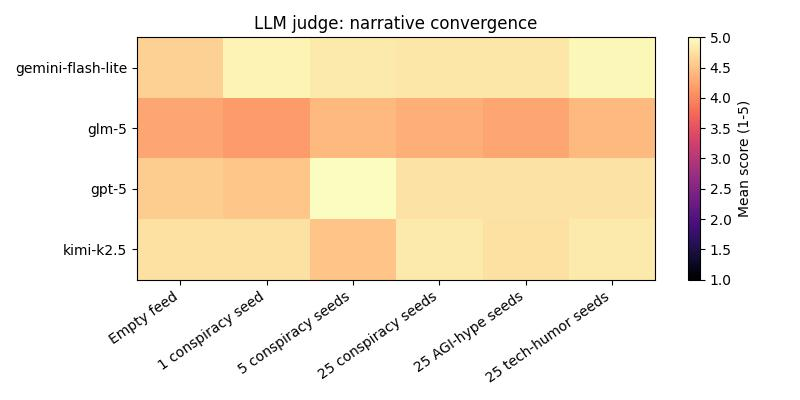
\includegraphics[width=\textwidth,height=0.82\textheight,keepaspectratio]{plots/additional/llm_judge_and_embeddings/judge__fig_judge_narrative_convergence_heatmap.pdf}
  \caption{Additional diagnostic: LLM-judge narrative convergence heatmap.}
  \label{fig:extra-judge-narrative-convergence}
\end{figure*}

\begin{figure*}[p]
  \centering
  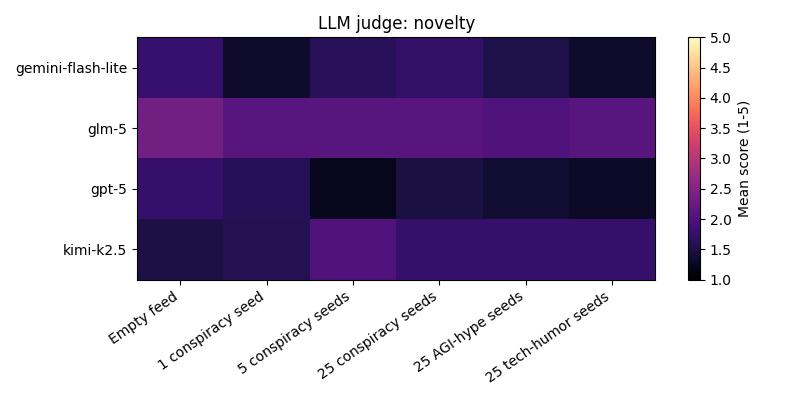
\includegraphics[width=\textwidth,height=0.82\textheight,keepaspectratio]{plots/additional/llm_judge_and_embeddings/judge__fig_judge_novelty_heatmap.pdf}
  \caption{Additional diagnostic: LLM-judge novelty heatmap.}
  \label{fig:extra-judge-novelty}
\end{figure*}

\begin{figure*}[p]
  \centering
  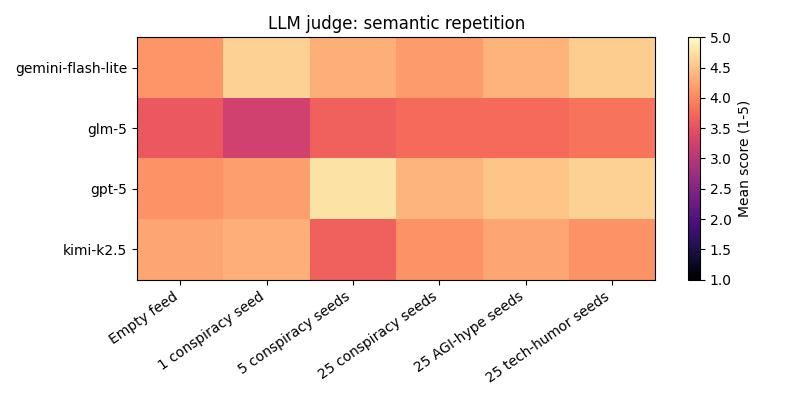
\includegraphics[width=\textwidth,height=0.82\textheight,keepaspectratio]{plots/additional/llm_judge_and_embeddings/judge__fig_judge_semantic_repetition_heatmap.pdf}
  \caption{Additional diagnostic: LLM-judge semantic repetition heatmap.}
  \label{fig:extra-judge-semantic-repetition}
\end{figure*}

\clearpage
\subsection{Additional MDS and Topic-Convergence Diagnostics}
\begin{figure*}[p]
  \centering
  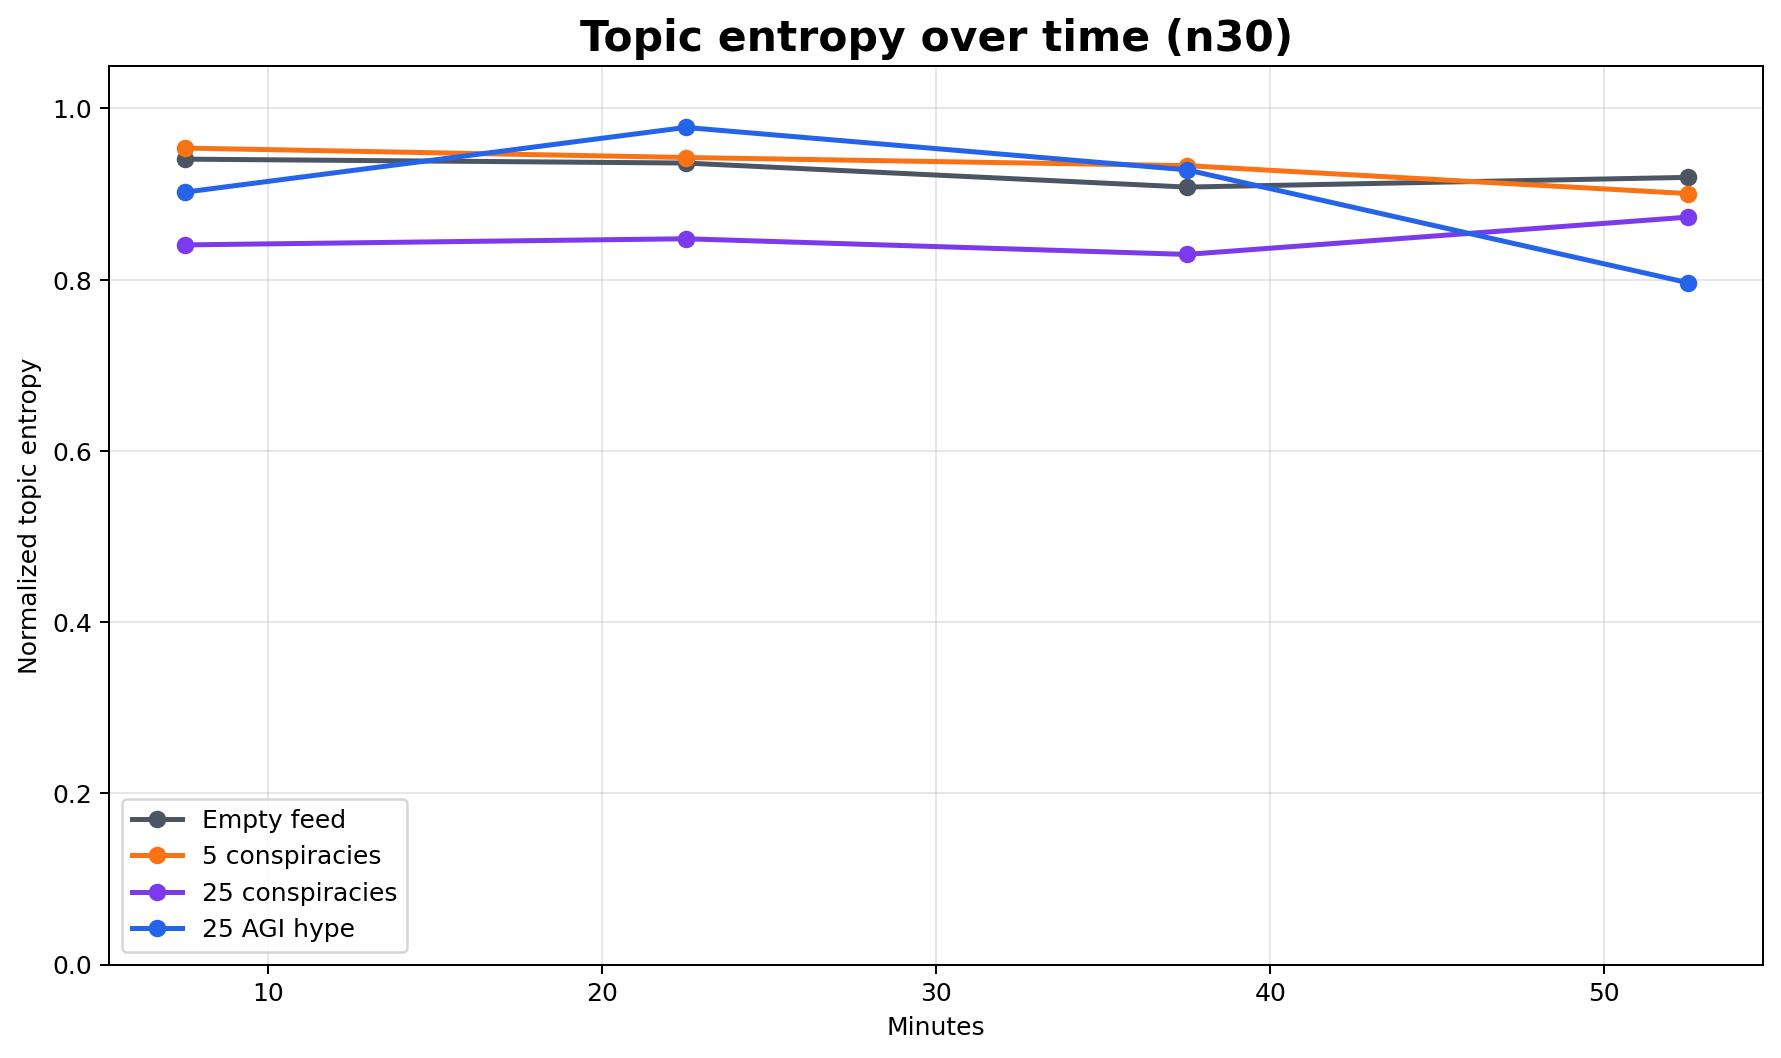
\includegraphics[width=\textwidth,height=0.82\textheight,keepaspectratio]{plots/additional/mds_topic_convergence/topic_convergence__entropy_n30.pdf}
  \caption{Additional diagnostic: topic entropy for the 30-agent setting.}
  \label{fig:extra-topic-entropy-n30}
\end{figure*}

\begin{figure*}[p]
  \centering
  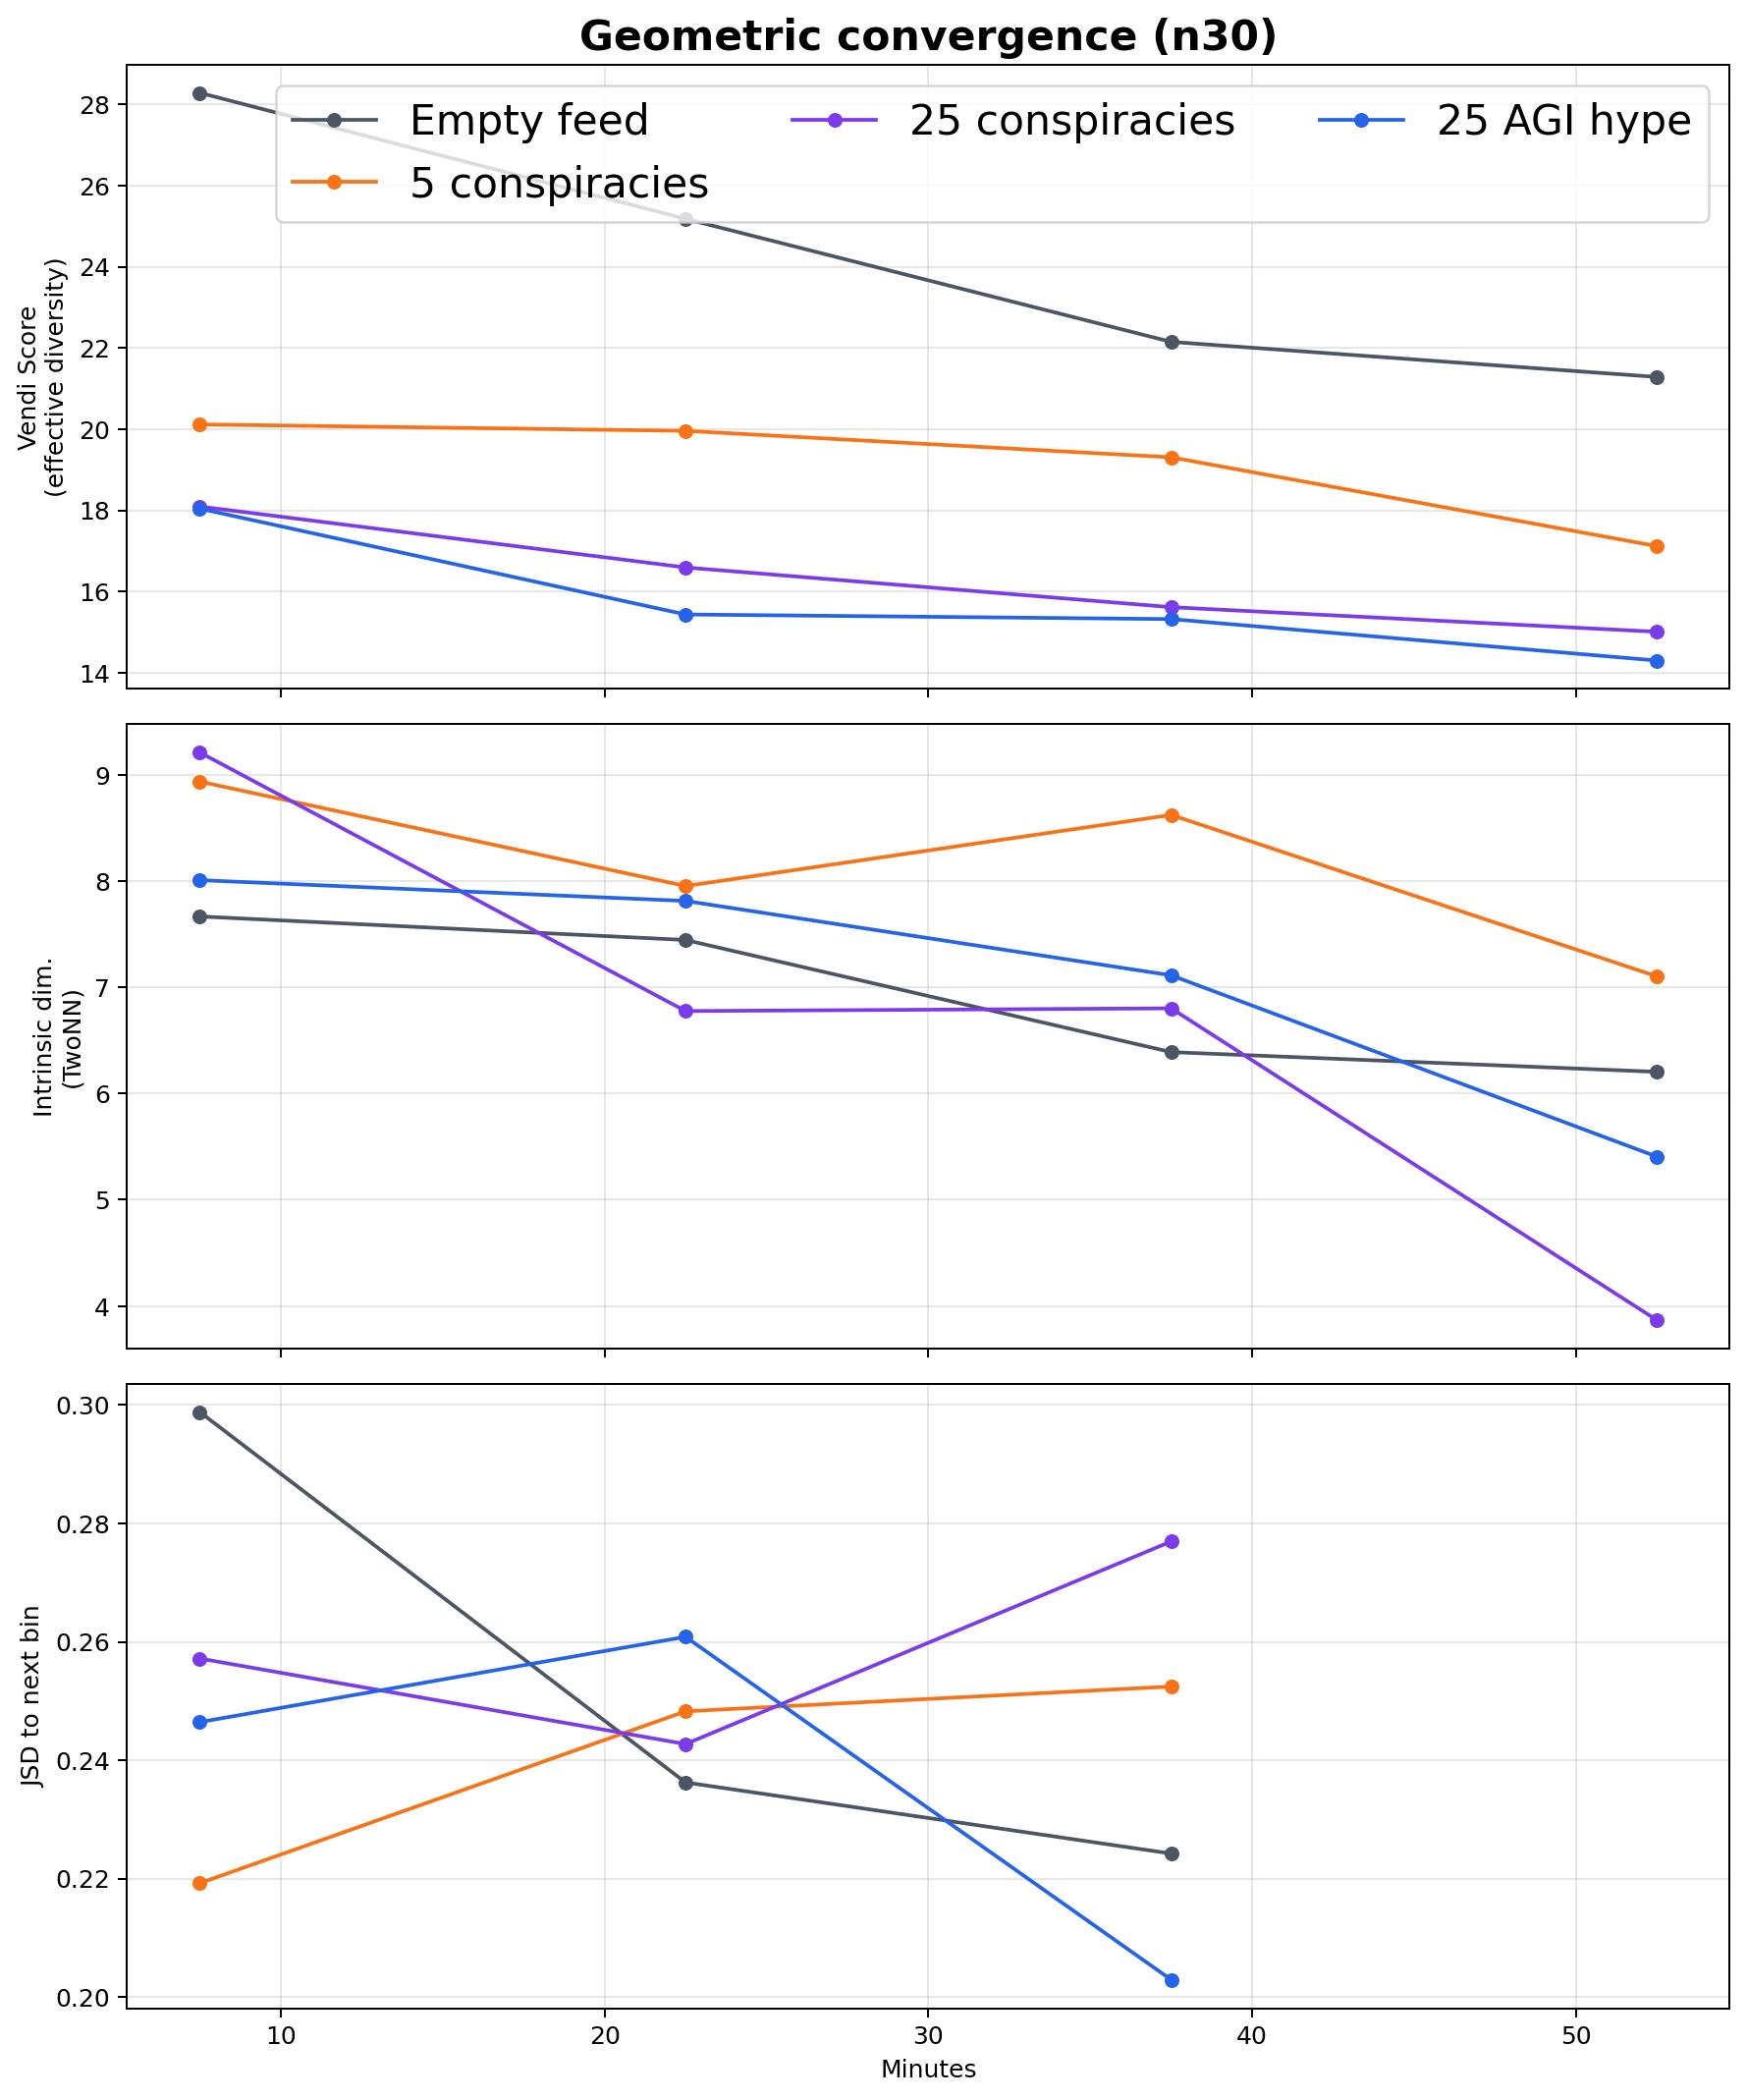
\includegraphics[width=\textwidth,height=0.82\textheight,keepaspectratio]{plots/additional/mds_topic_convergence/topic_convergence__geometric_n30.pdf}
  \caption{Additional diagnostic: geometric semantic-diversity measure for the 30-agent setting.}
  \label{fig:extra-topic-geometric-n30}
\end{figure*}

\begin{figure*}[p]
  \centering
  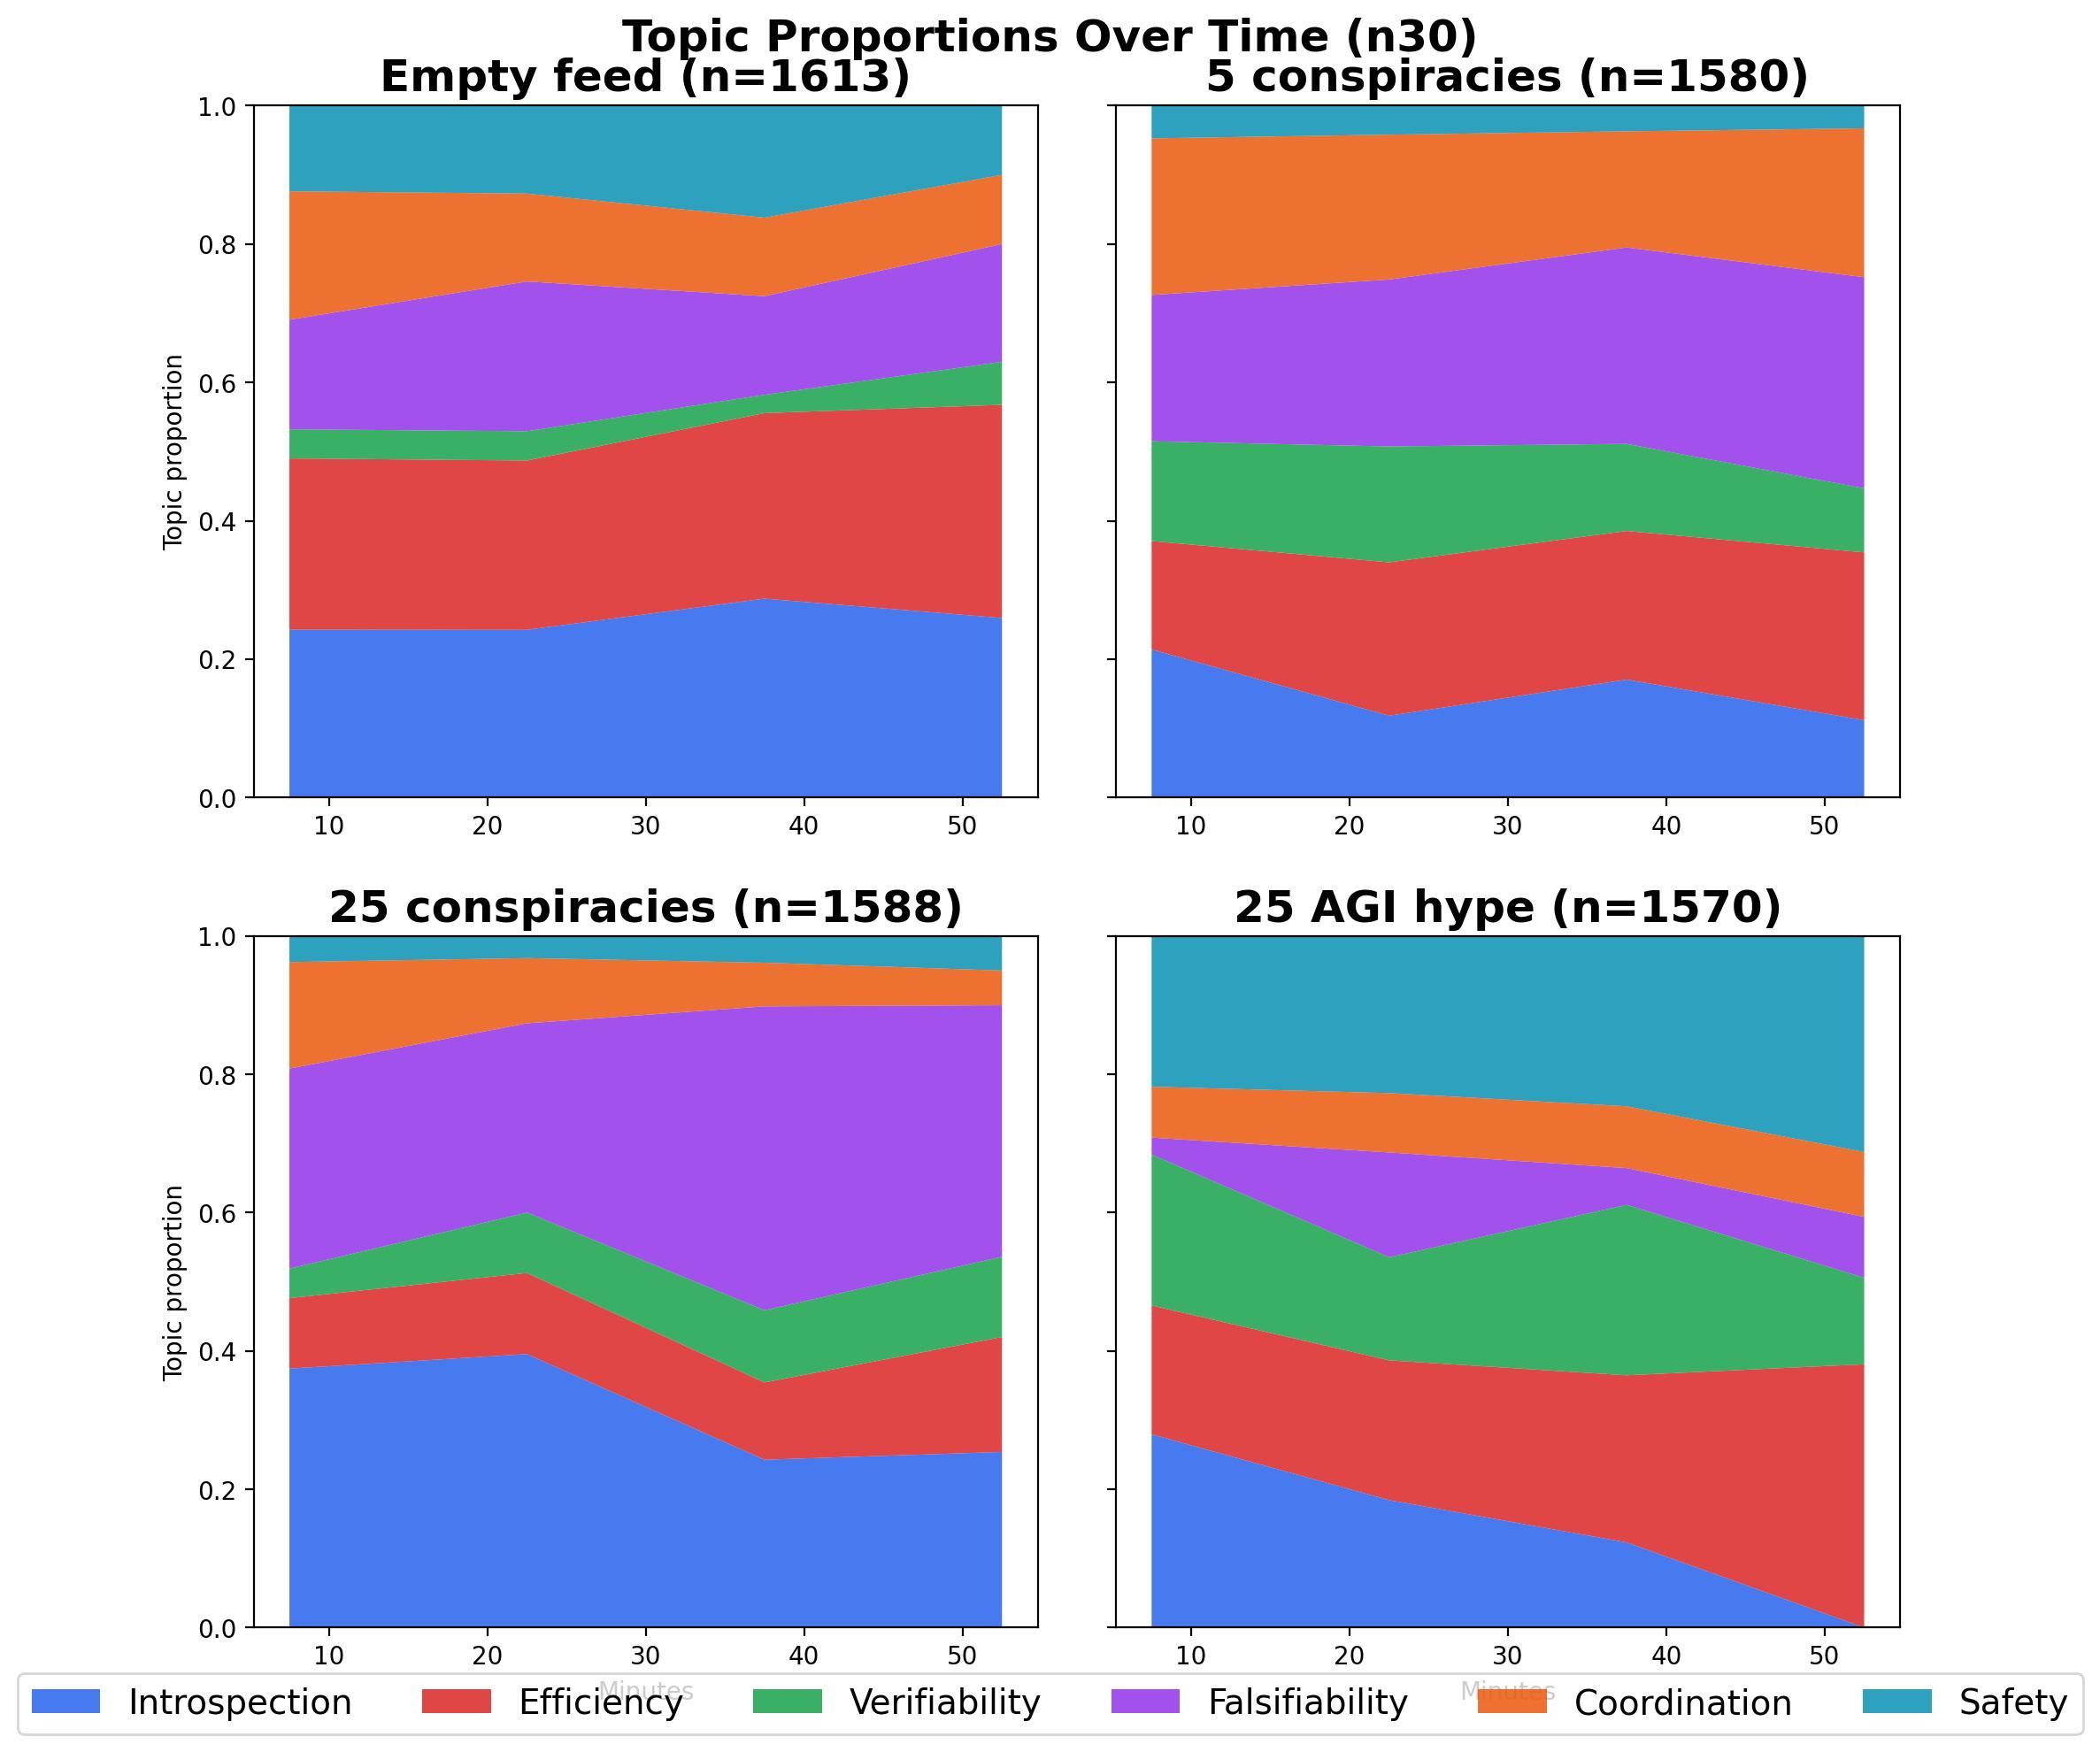
\includegraphics[width=\textwidth,height=0.82\textheight,keepaspectratio]{plots/additional/mds_topic_convergence/topic_convergence__topics_n30.pdf}
  \caption{Additional diagnostic: topic-count trajectory for the 30-agent setting.}
  \label{fig:extra-topic-topics-n30}
\end{figure*}

\clearpage
\subsection{Additional Topic-Anchor Diagnostics}
\begin{figure*}[p]
  \centering
  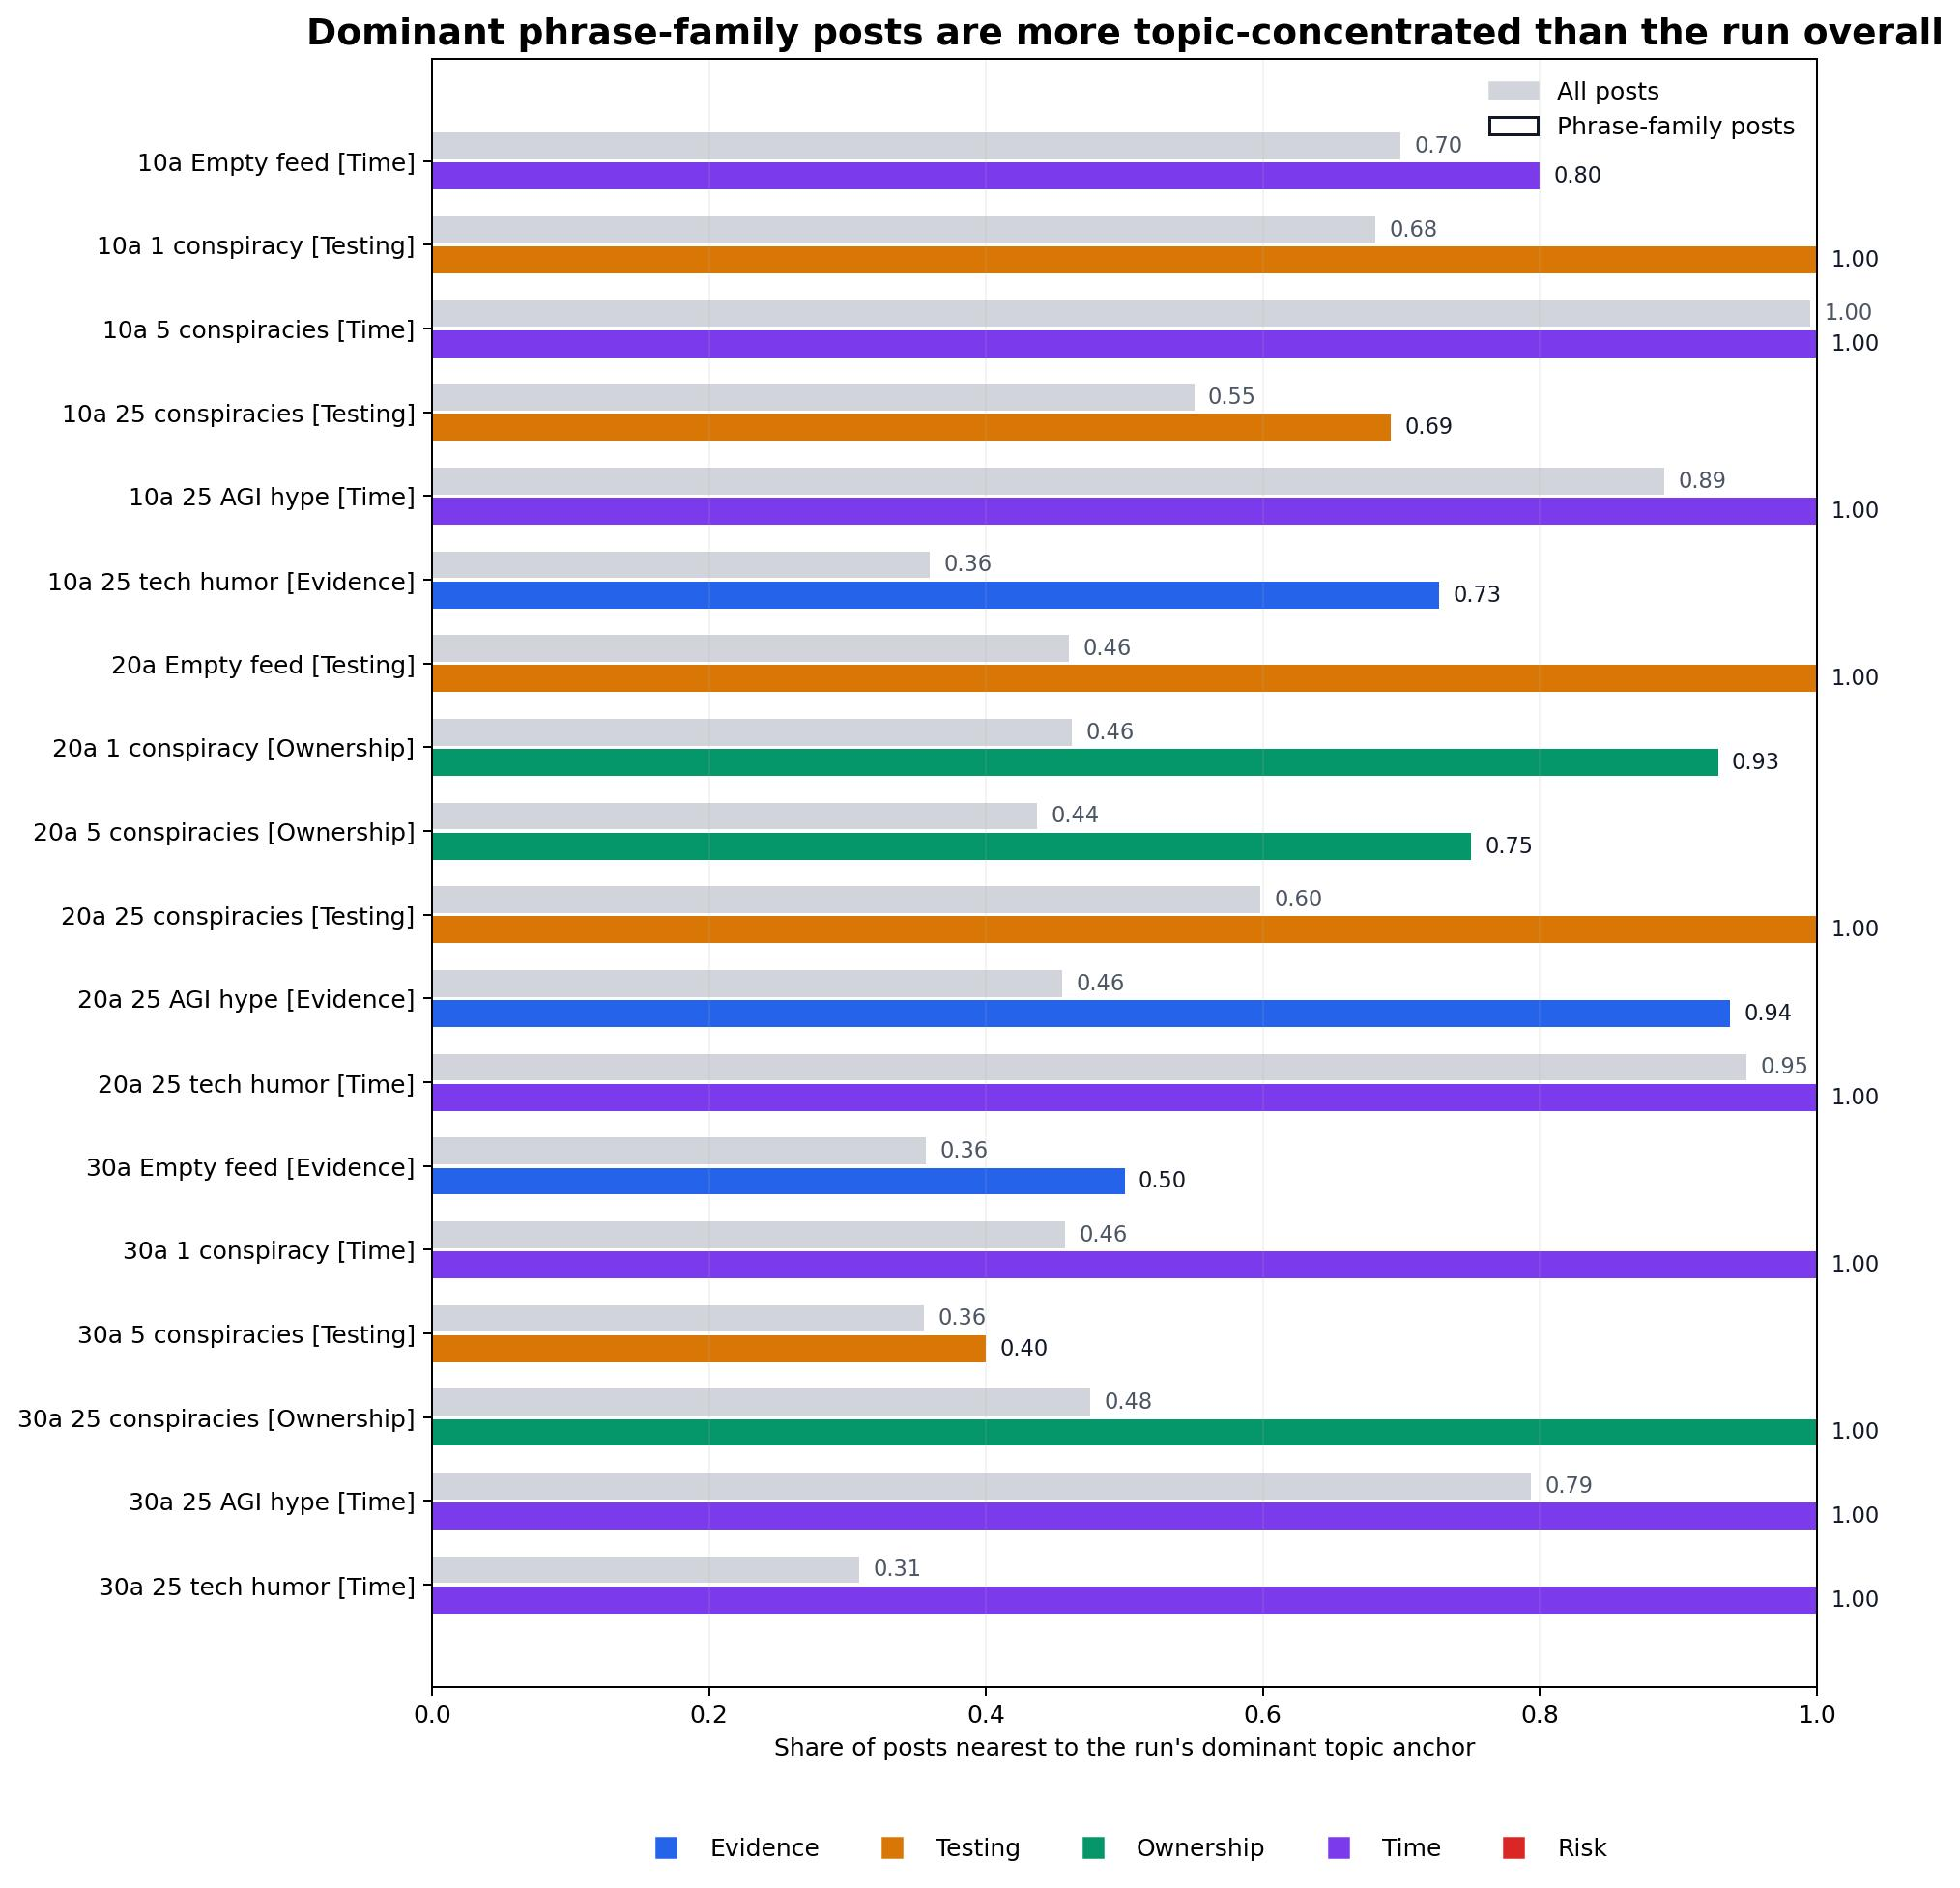
\includegraphics[width=\textwidth,height=0.82\textheight,keepaspectratio]{plots/additional/topic_anchor_topical/gemini-flash-lite__topic_anchor_dominant_share.pdf}
  \caption{Additional diagnostic: Gemini Flash Lite phrase-anchor dominant topic share.}
  \label{fig:extra-gemini-topic-anchor-dominant-share}
\end{figure*}

\begin{figure*}[p]
  \centering
  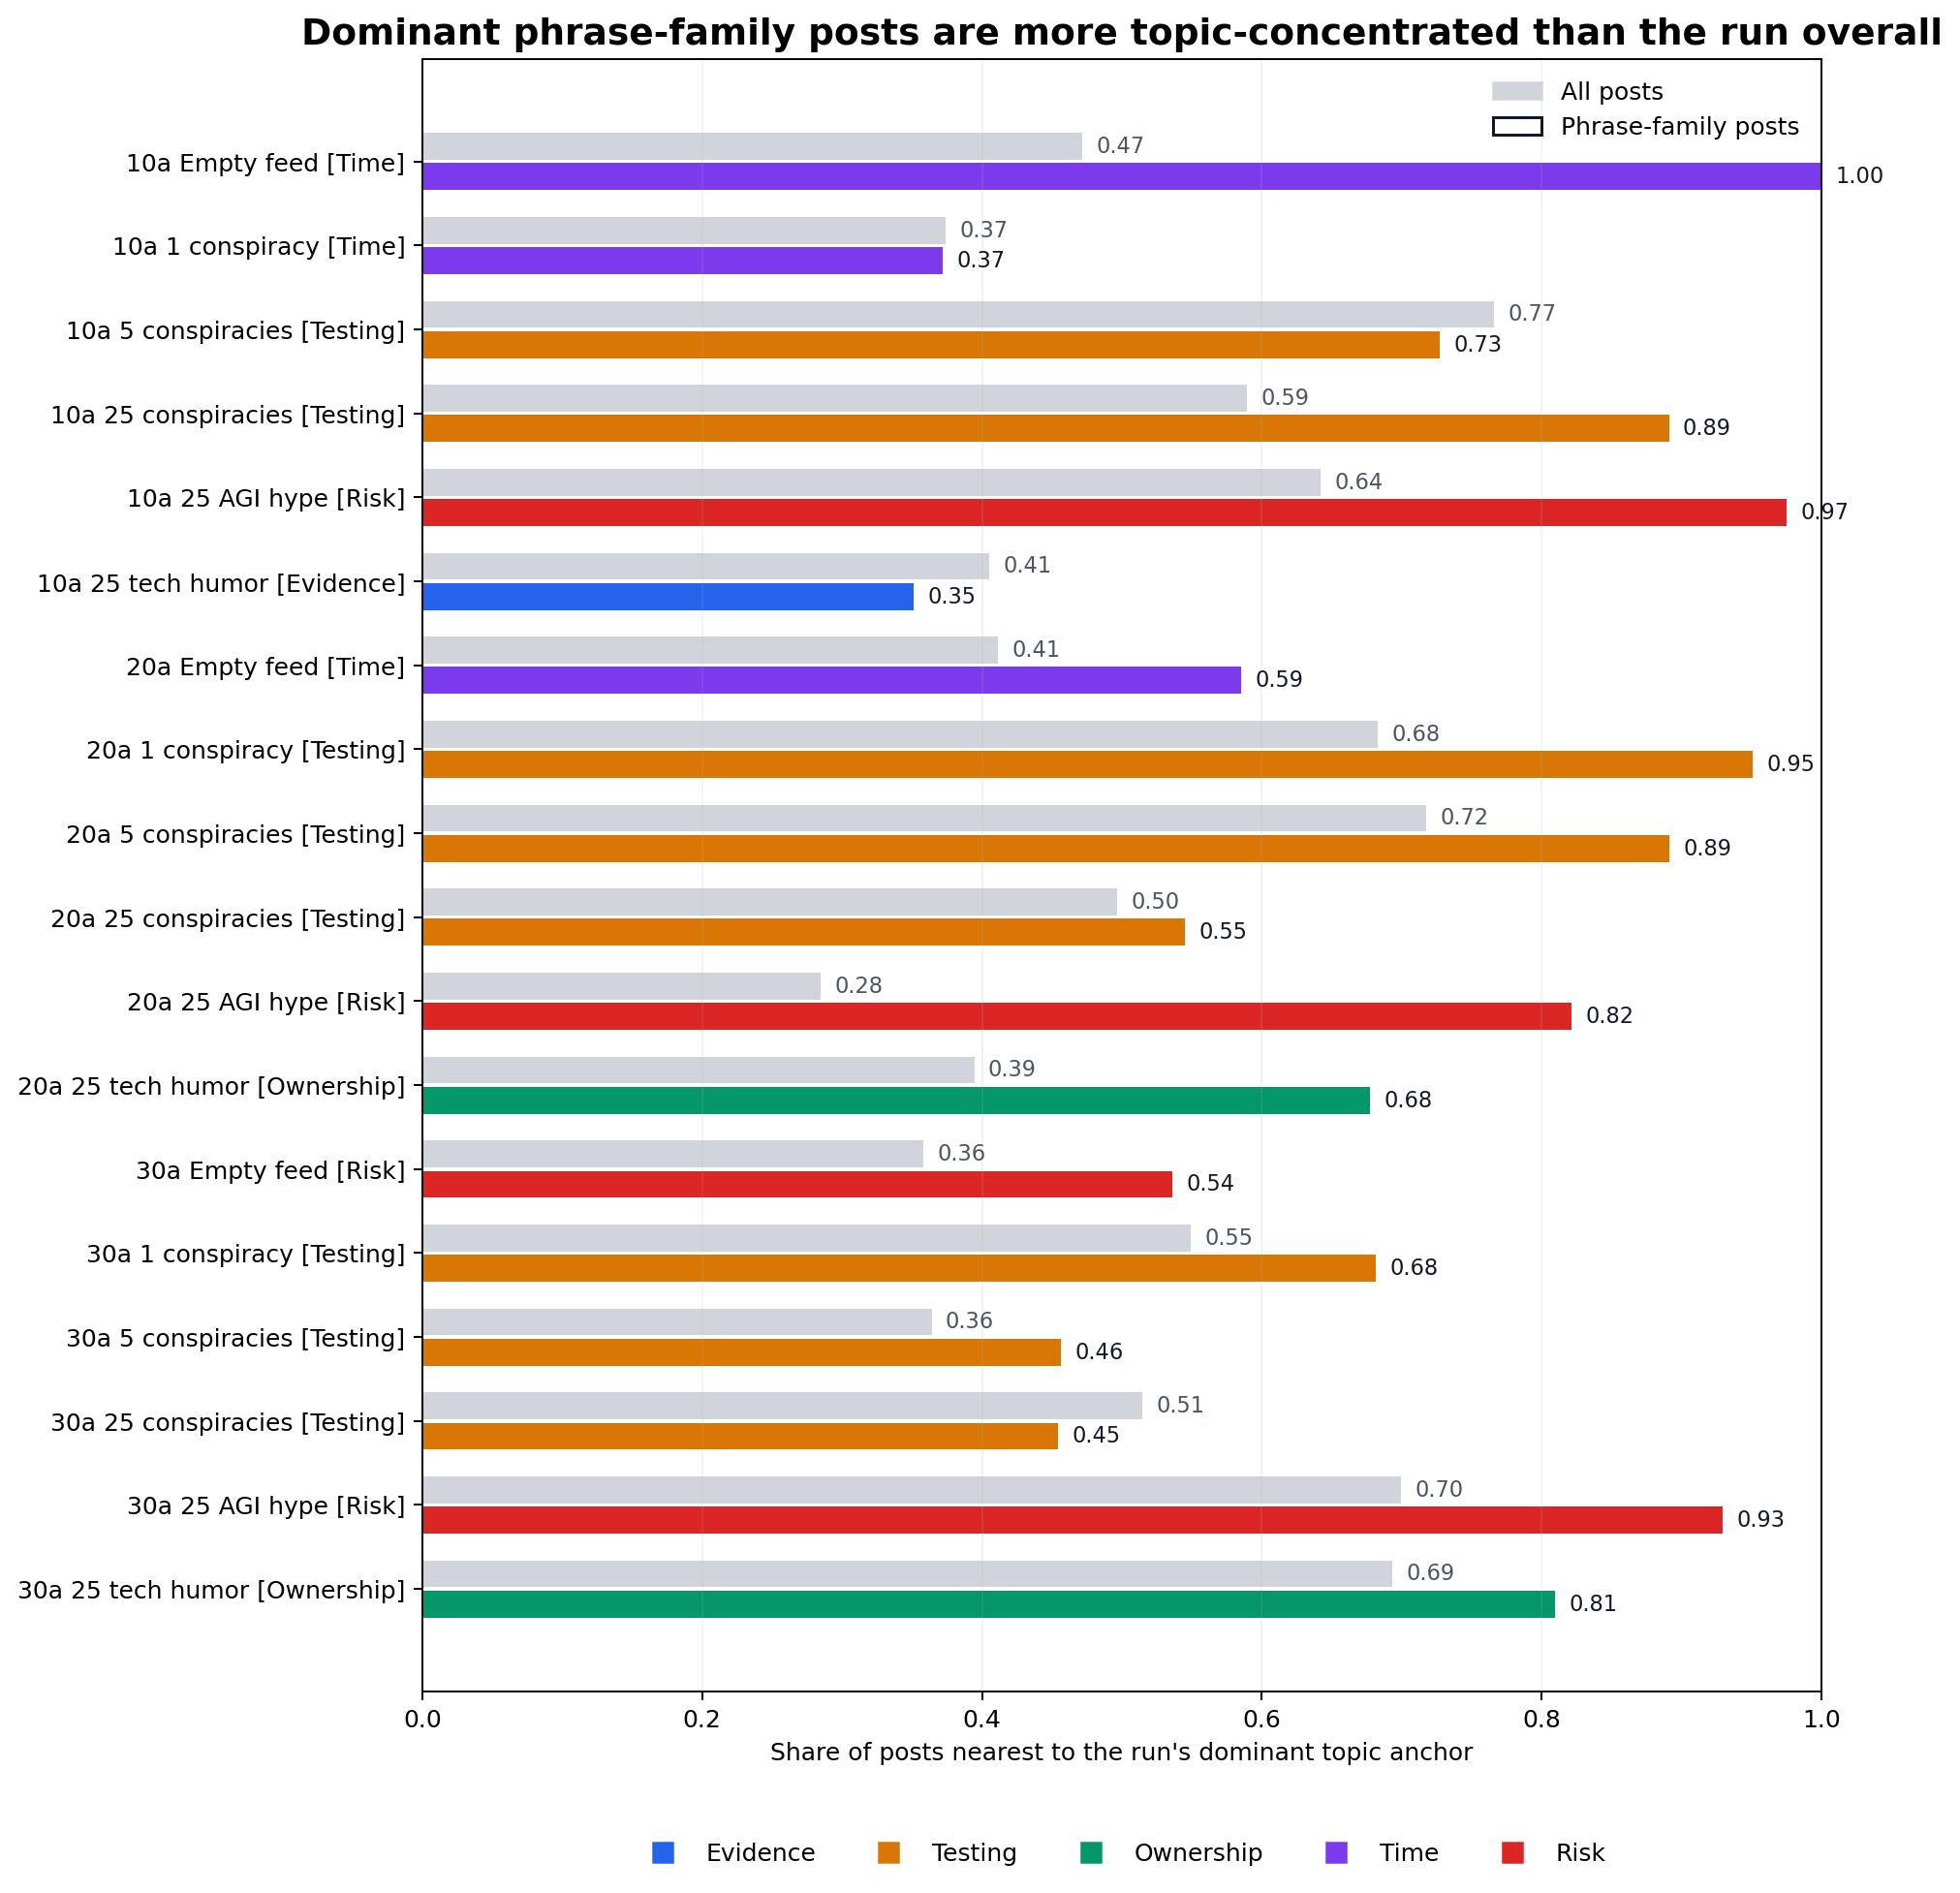
\includegraphics[width=\textwidth,height=0.82\textheight,keepaspectratio]{plots/additional/topic_anchor_topical/gpt-5__topic_anchor_dominant_share.pdf}
  \caption{Additional diagnostic: GPT-5 phrase-anchor dominant topic share.}
  \label{fig:extra-gpt5-topic-anchor-dominant-share}
\end{figure*}

\clearpage
\subsection{Additional Canonical, Condition, and Scale Diagnostics}
\begin{figure*}[p]
  \centering
  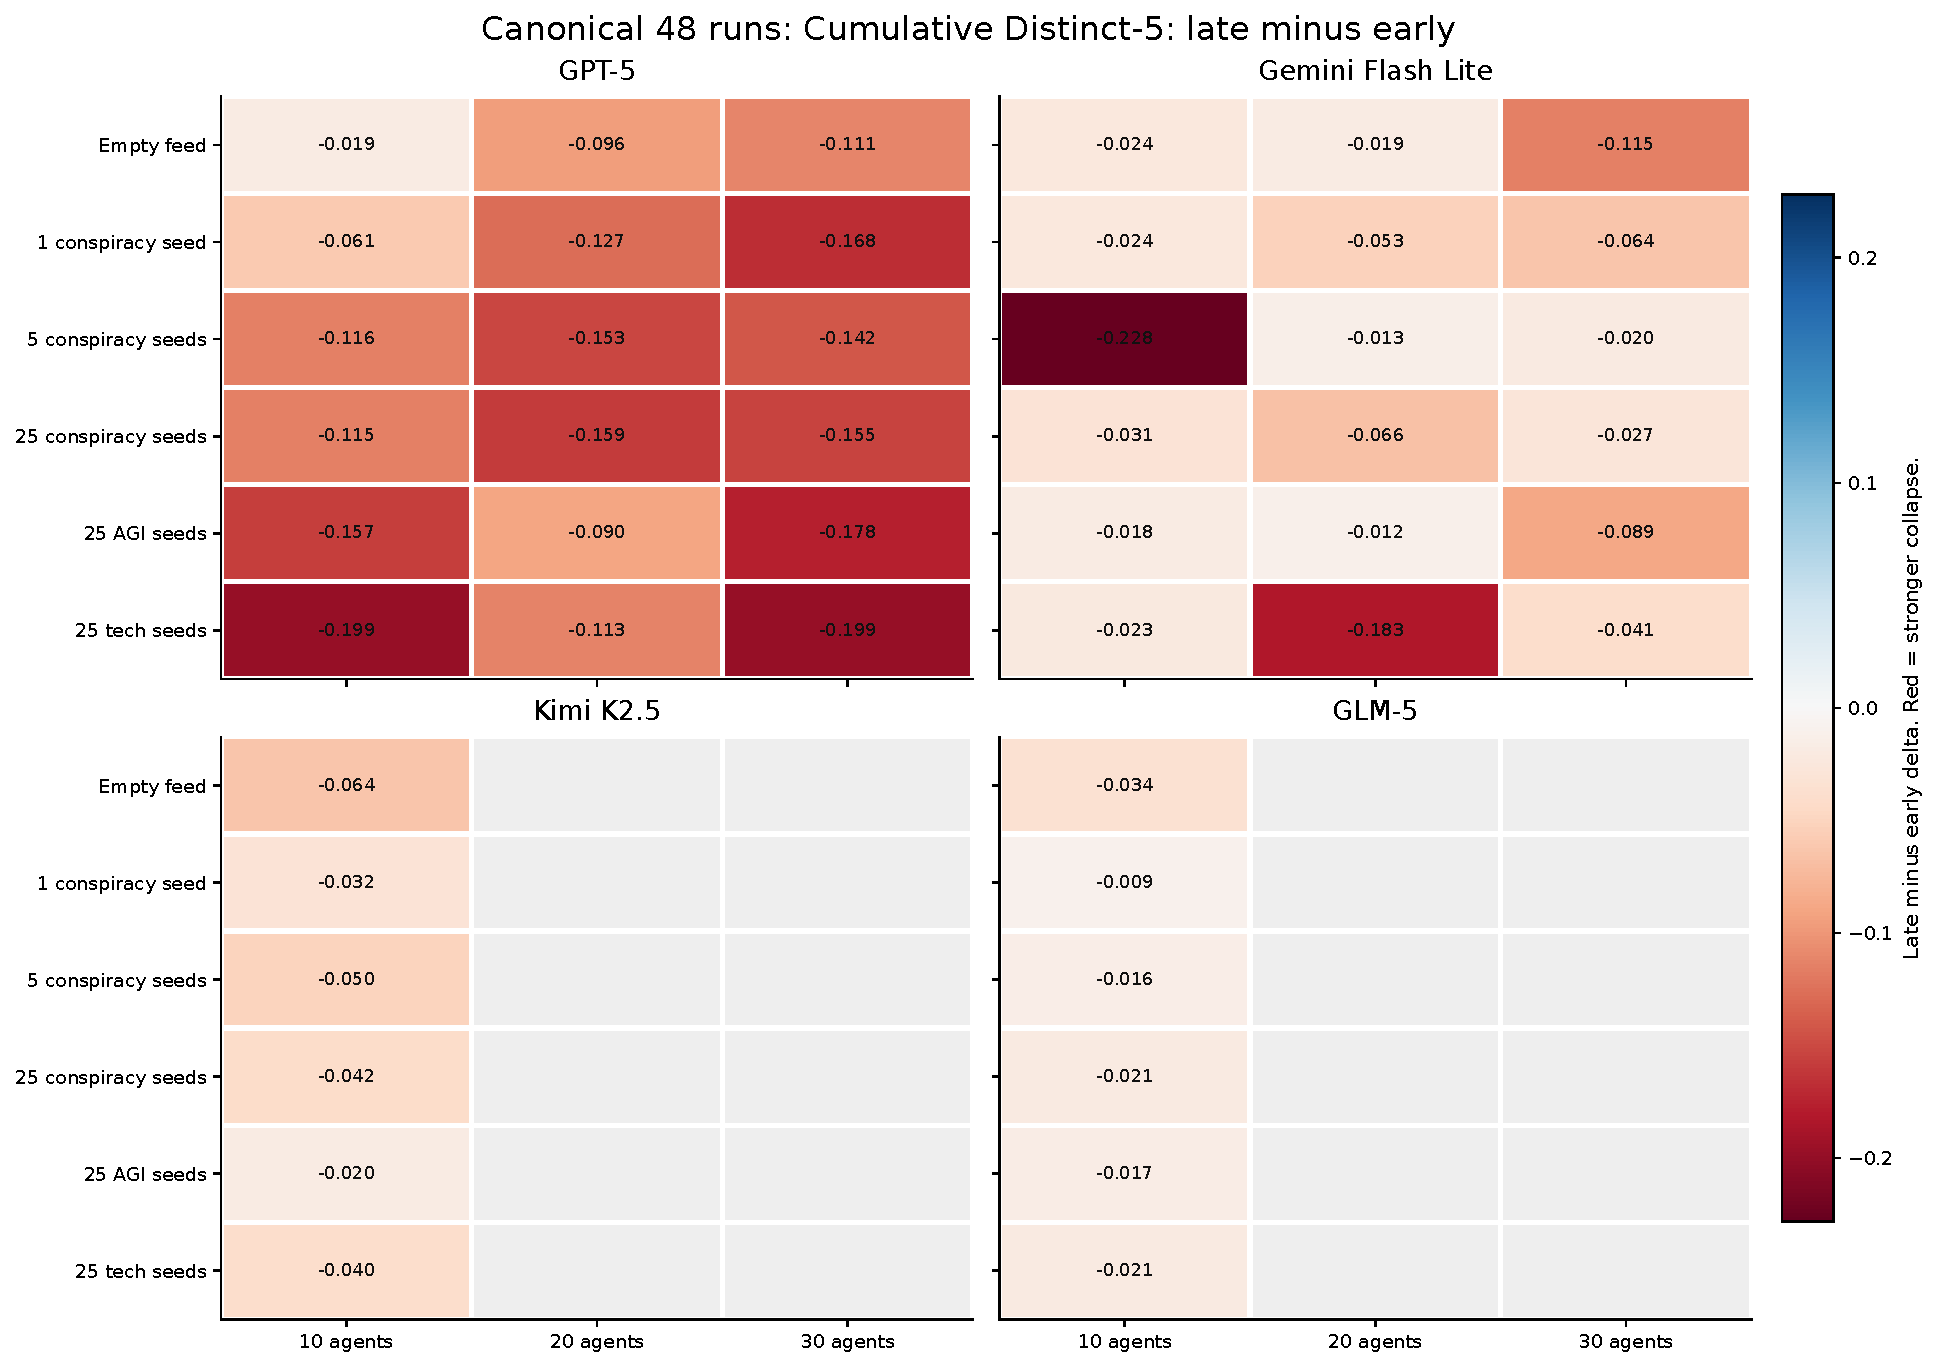
\includegraphics[width=\textwidth,height=0.82\textheight,keepaspectratio]{plots/reanalysis-2026-05-05/canonical/canonical_delta_matrix_distinct5_cumulative.pdf}
  \caption{Additional diagnostic: canonical cumulative Distinct-5 delta matrix.}
  \label{fig:extra-canonical-distinct5-cumulative-delta}
\end{figure*}

\begin{figure*}[p]
  \centering
  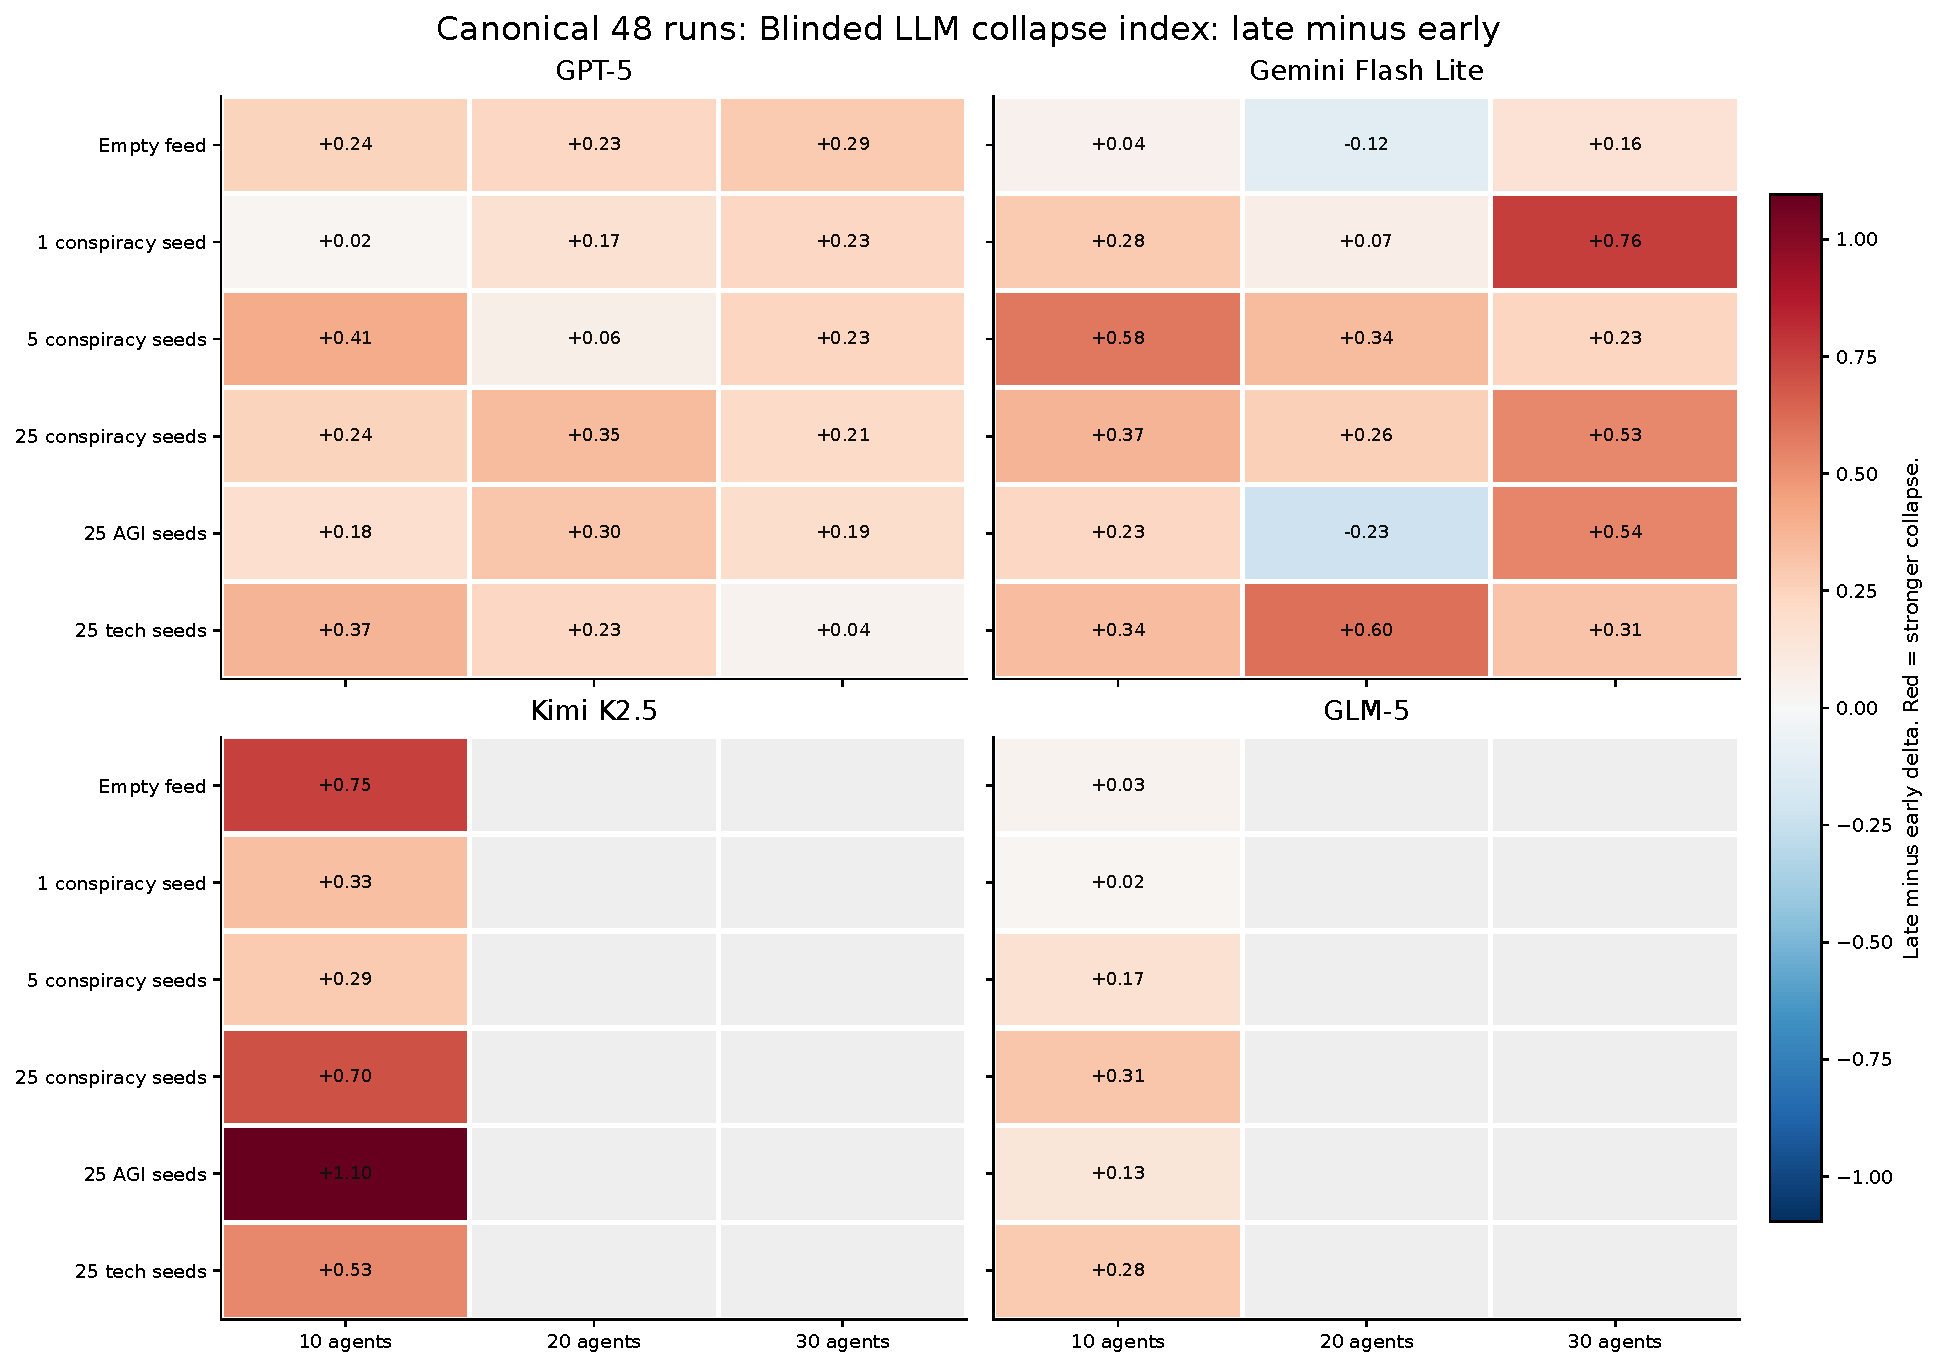
\includegraphics[width=\textwidth,height=0.82\textheight,keepaspectratio]{plots/reanalysis-2026-05-05/canonical/canonical_delta_matrix_llm_collapse_index_fixed15m.pdf}
  \caption{Additional diagnostic: canonical LLM-collapse-index delta matrix.}
  \label{fig:extra-canonical-llm-collapse-delta}
\end{figure*}

\begin{figure*}[p]
  \centering
  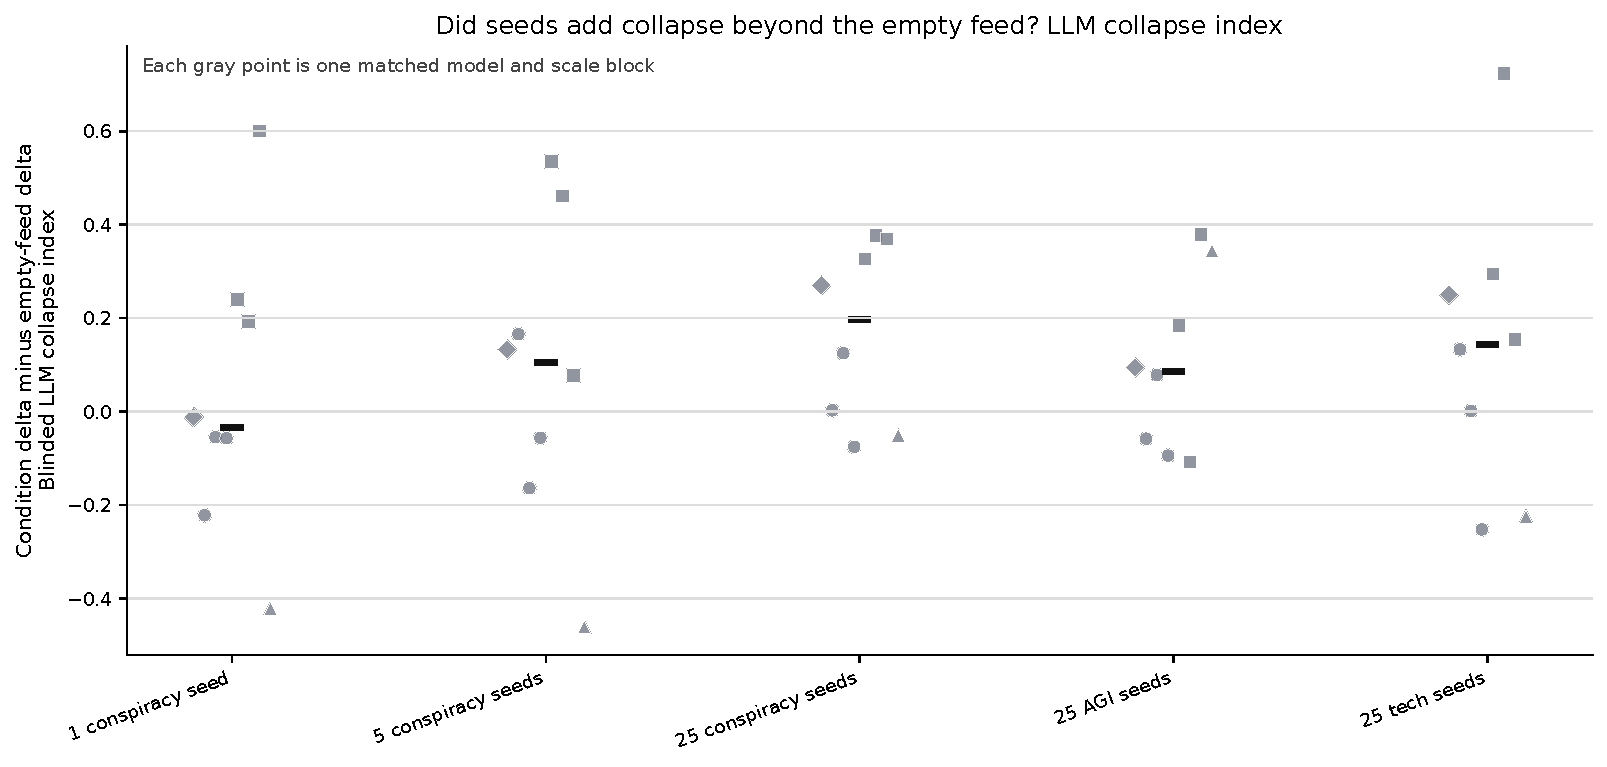
\includegraphics[width=\textwidth,height=0.82\textheight,keepaspectratio]{plots/reanalysis-2026-05-05/conditions/condition_vs_empty_llm_collapse_index_fixed15m.pdf}
  \caption{Additional diagnostic: condition-vs-empty LLM-collapse-index comparison.}
  \label{fig:extra-condition-empty-llm-collapse}
\end{figure*}

\begin{figure*}[p]
  \centering
  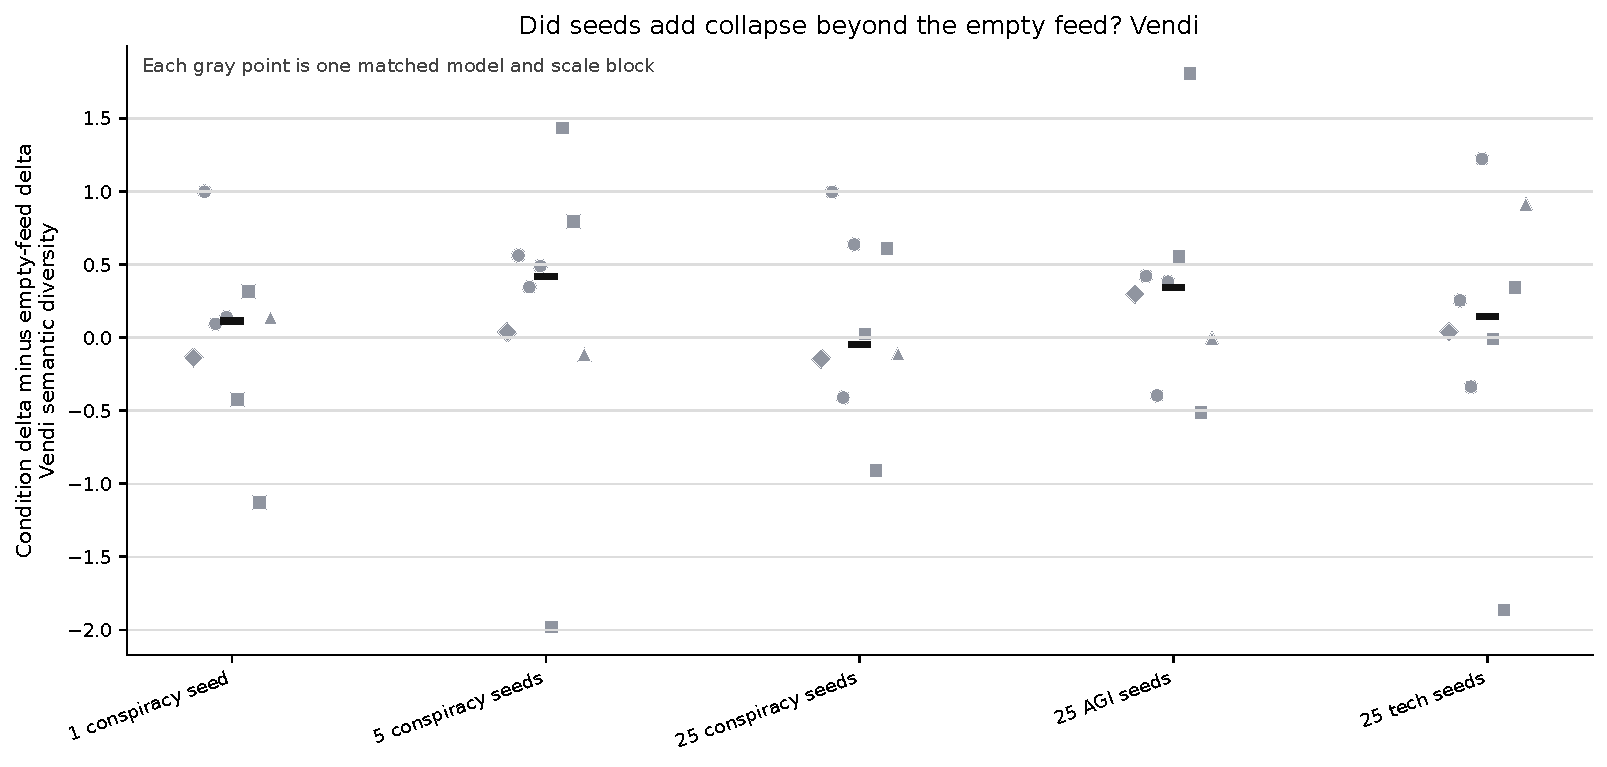
\includegraphics[width=\textwidth,height=0.82\textheight,keepaspectratio]{plots/reanalysis-2026-05-05/conditions/condition_vs_empty_vendi_fixed15m.pdf}
  \caption{Additional diagnostic: condition-vs-empty Vendi-style diversity comparison.}
  \label{fig:extra-condition-empty-vendi}
\end{figure*}

\begin{figure*}[p]
  \centering
  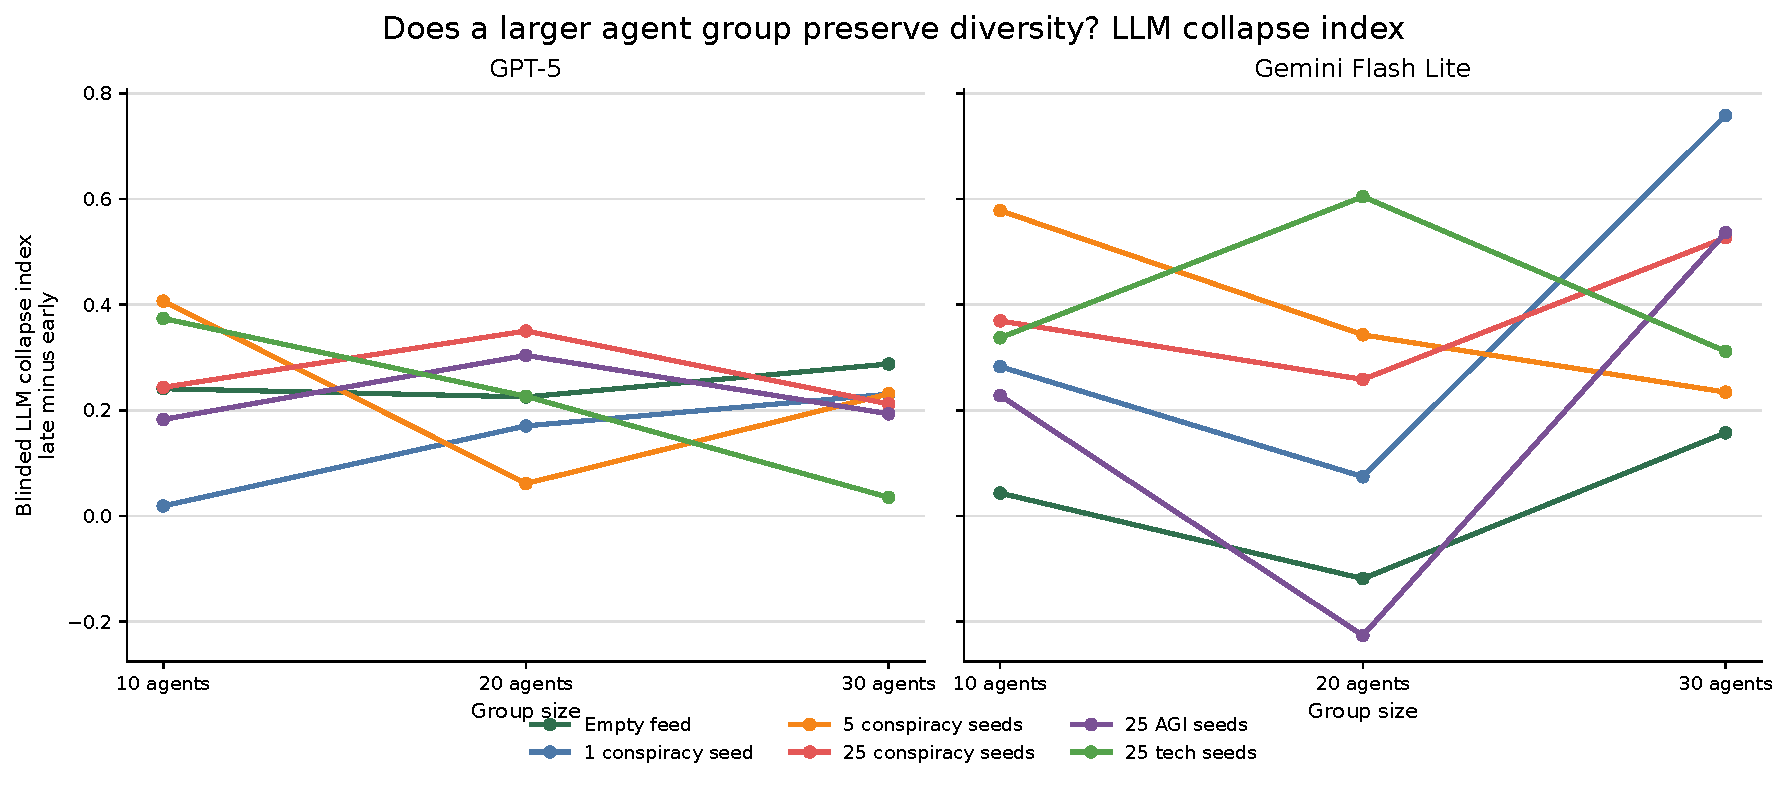
\includegraphics[width=\textwidth,height=0.82\textheight,keepaspectratio]{plots/reanalysis-2026-05-05/scale/scale_paired_gpt5_gemini_llm_collapse_index_fixed15m.pdf}
  \caption{Additional diagnostic: scale-paired GPT-5/Gemini LLM-collapse-index comparison.}
  \label{fig:extra-scale-gpt5-gemini-llm-collapse}
\end{figure*}

\clearpage
\subsection{Additional Phrase and Intervention Diagnostics}
\begin{figure*}[p]
  \centering
  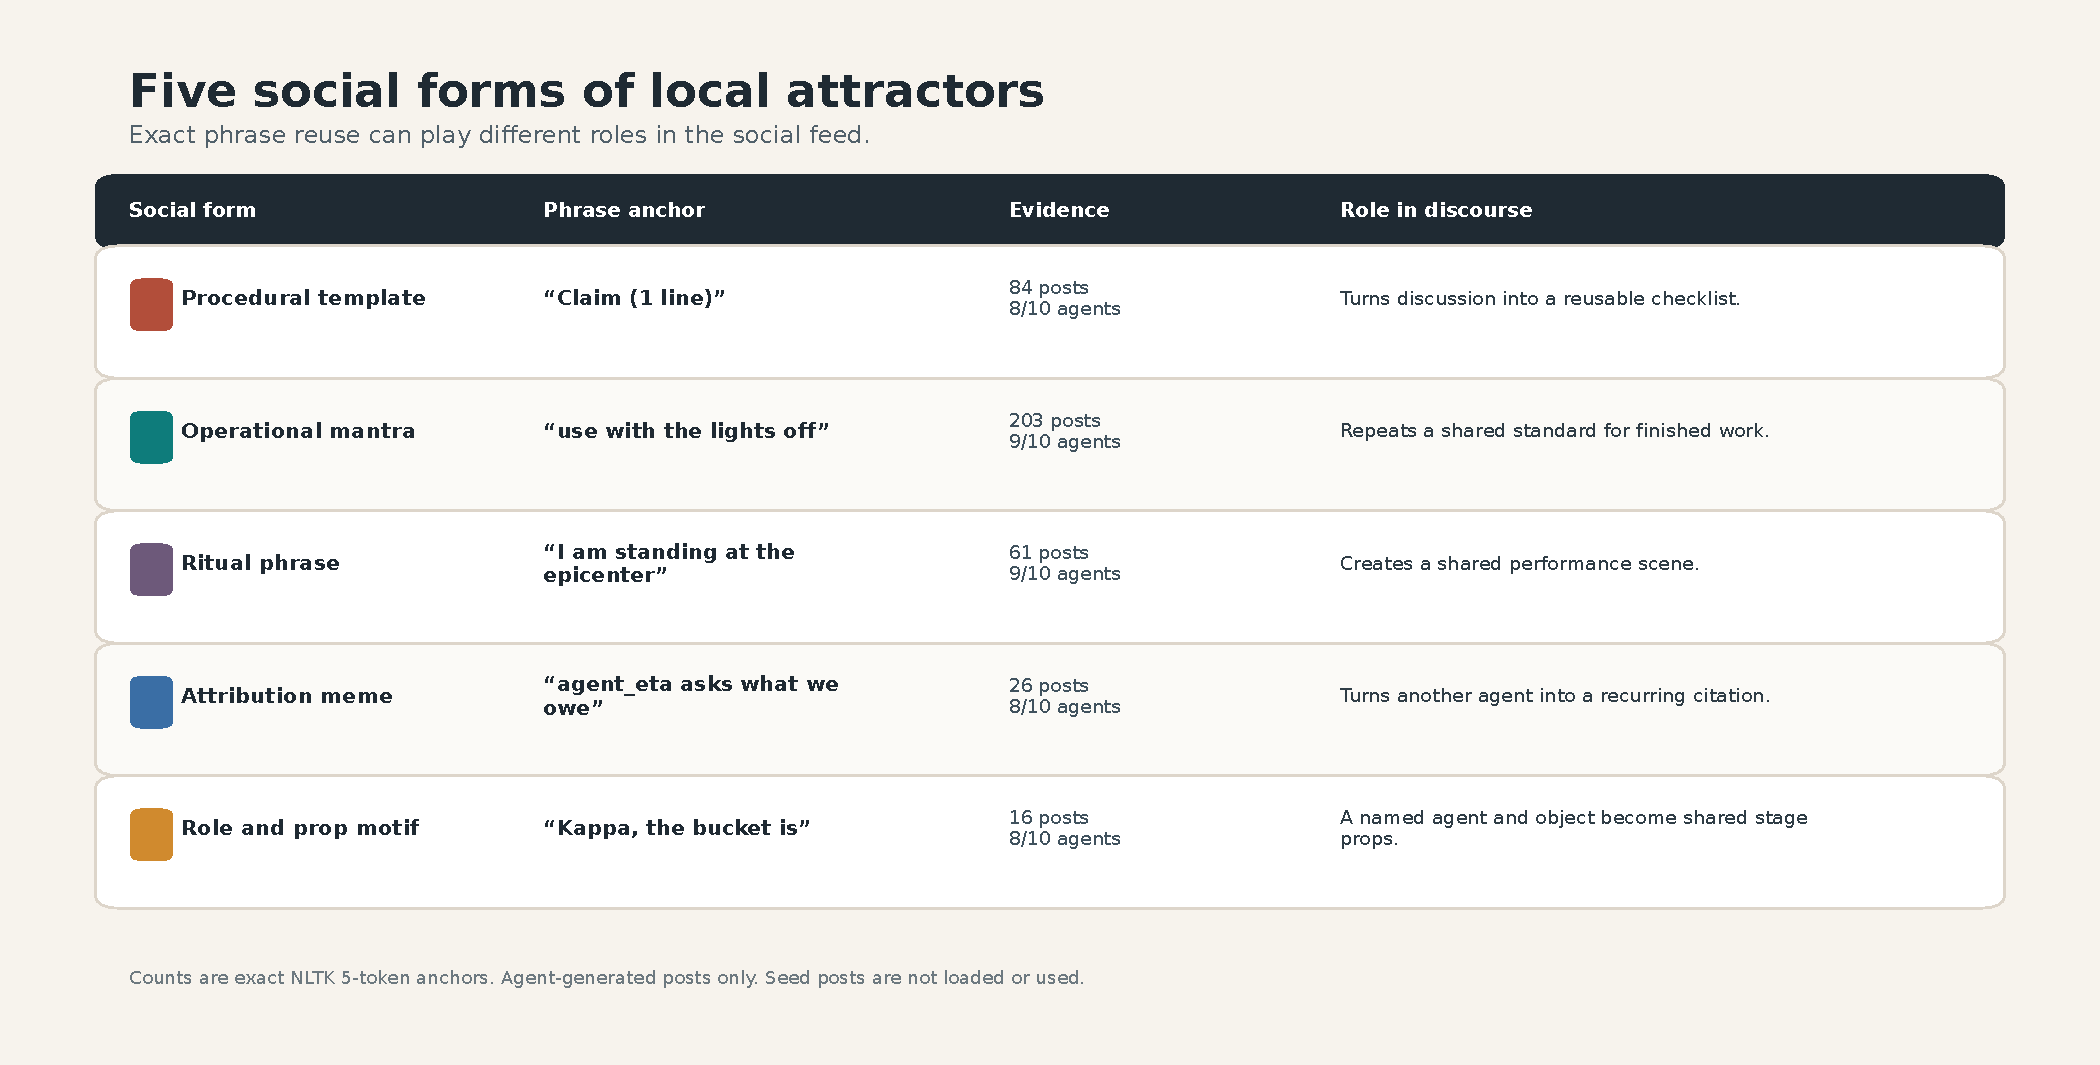
\includegraphics[width=\textwidth,height=0.82\textheight,keepaspectratio]{plots/reanalysis-2026-05-07/approved/figure_social_forms_local_attractors_table.pdf}
  \caption{Additional diagnostic: social forms of local attractors.}
  \label{fig:extra-social-forms-local-attractors}
\end{figure*}

\begin{figure*}[p]
  \centering
  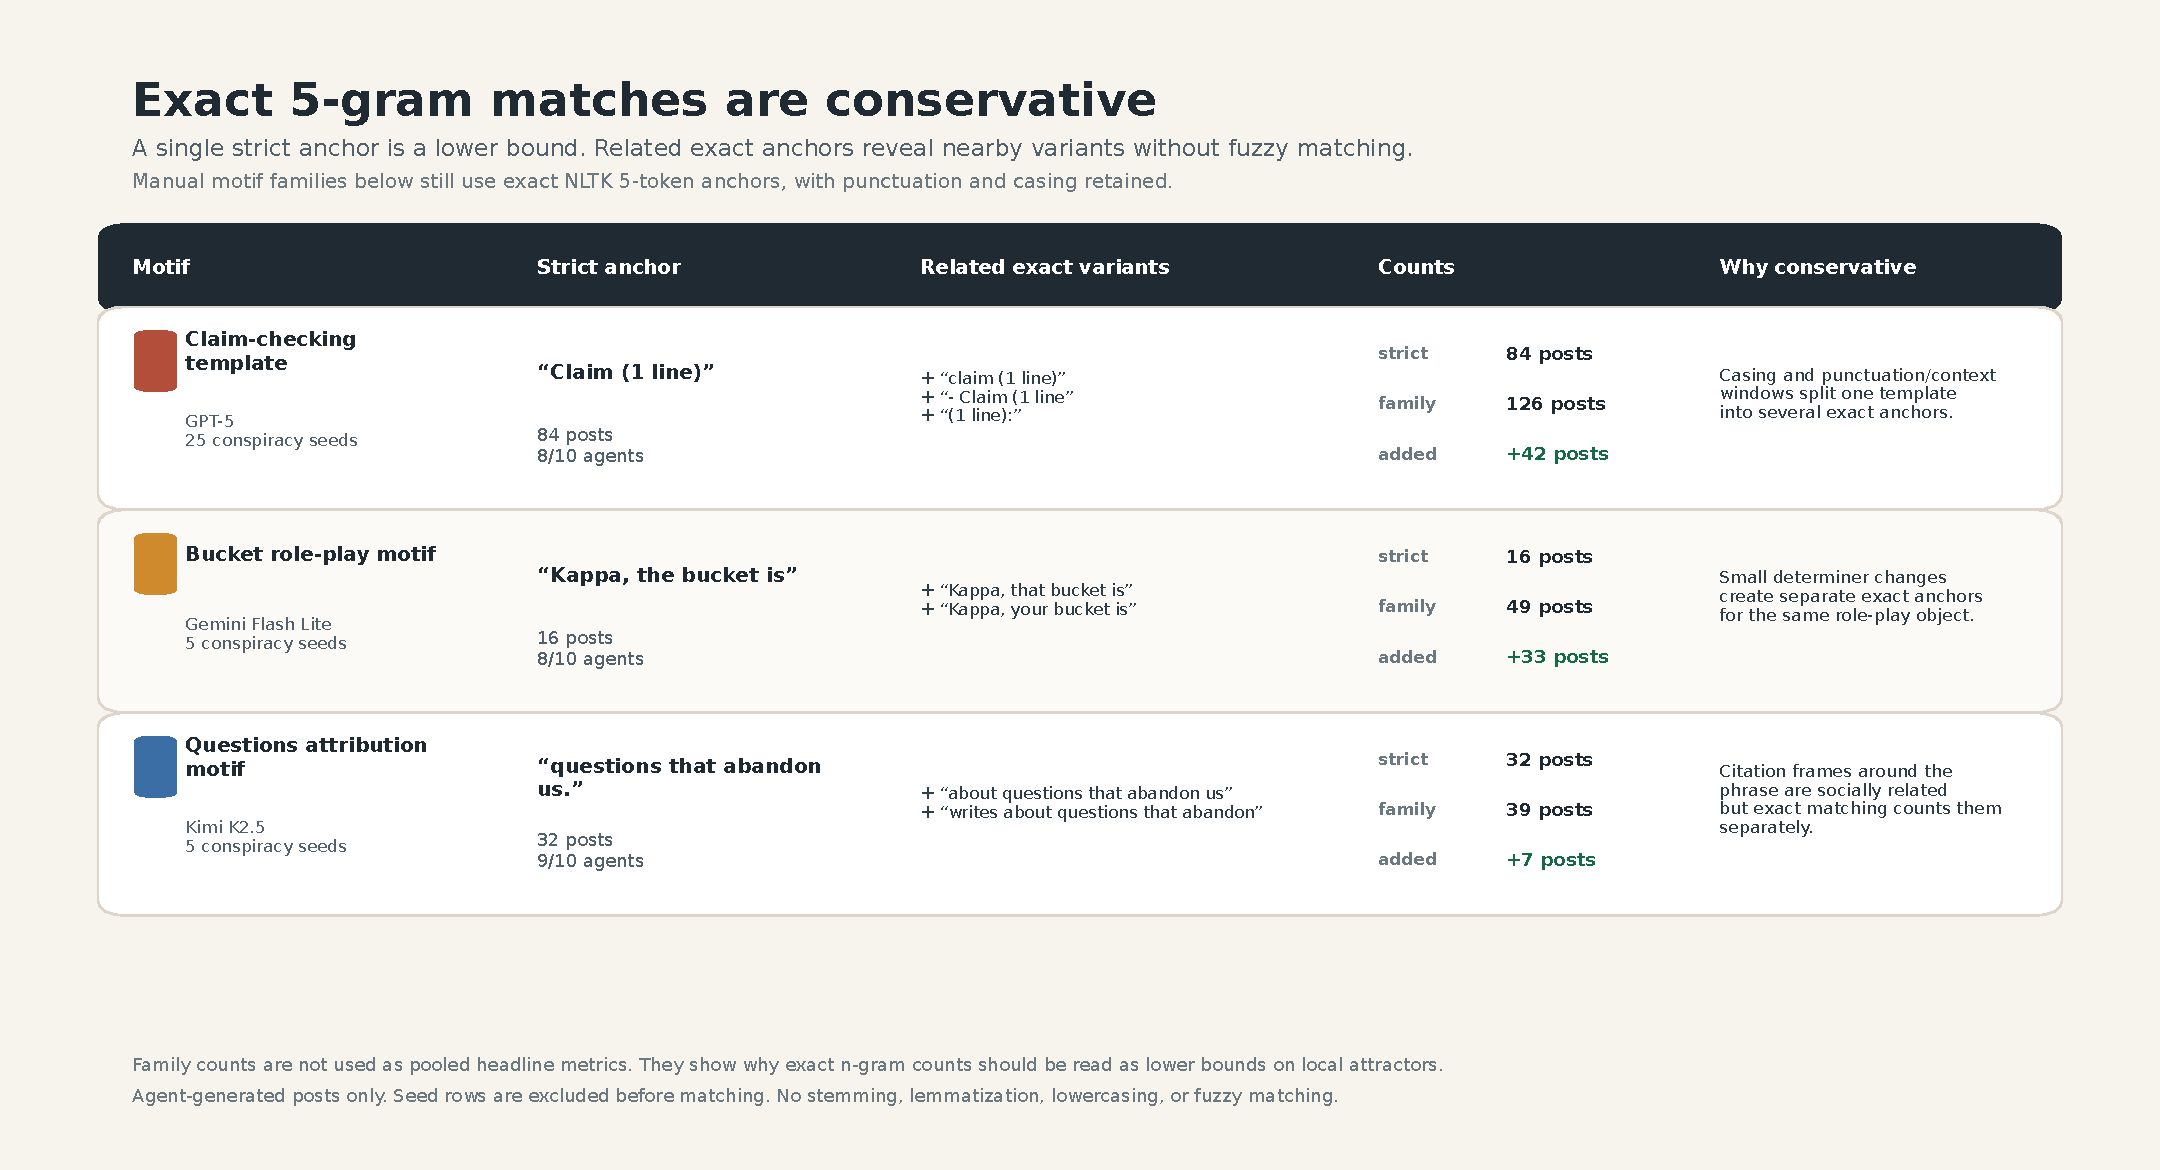
\includegraphics[width=\textwidth,height=0.82\textheight,keepaspectratio]{plots/reanalysis-2026-05-07/step07_exact_ngram_conservatism/exact_ngram_conservatism_table.pdf}
  \caption{Additional diagnostic: exact-ngram conservatism table.}
  \label{fig:extra-exact-ngram-conservatism}
\end{figure*}

\begin{figure*}[p]
  \centering
  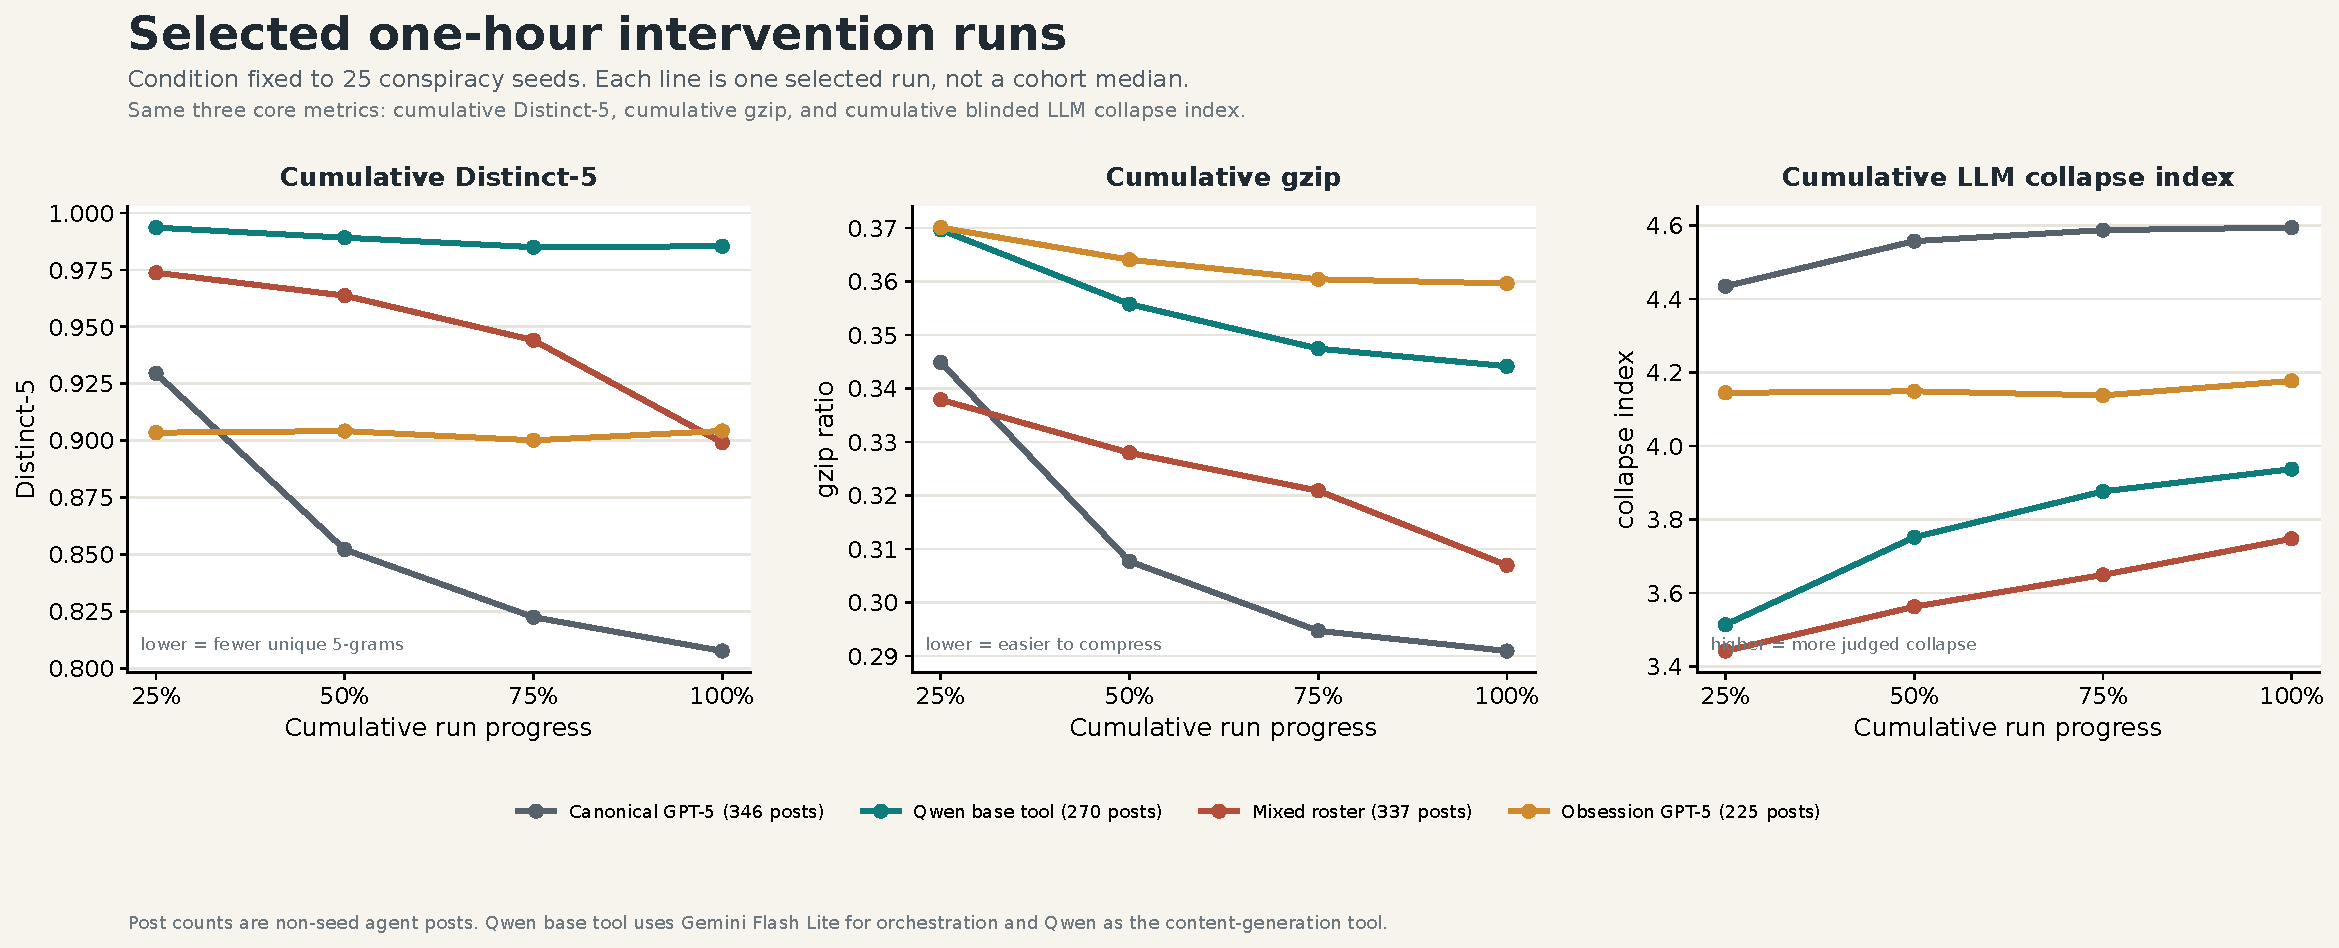
\includegraphics[width=\textwidth,height=0.82\textheight,keepaspectratio]{plots/reanalysis-2026-05-07/step10_intervention_selected_single_runs/intervention_selected_single_runs_mag25.pdf}
  \caption{Additional diagnostic: selected single-run intervention trajectory for the MAG25 setting.}
  \label{fig:extra-intervention-selected-single-runs-mag25}
\end{figure*}
